%%%%%%%%%%%%%%%%%%%%%%%%%%%%%%%%%%%%%%%%%
% Beamer Presentation
% LaTeX Template
% Version 1.0 (10/11/12)
%
% This template has been downloaded from:
% http://www.LaTeXTemplates.com
%
% License:
% CC BY-NC-SA 3.0 (http://creativecommons.org/licenses/by-nc-sa/3.0/)
%
%%%%%%%%%%%%%%%%%%%%%%%%%%%%%%%%%%%%%%%%%

%----------------------------------------------------------------------------------------
%	PACKAGES AND THEMES
%----------------------------------------------------------------------------------------

\documentclass{beamer}

\mode<presentation> {

% The Beamer class comes with a number of default slide themes
% which change the colors and layouts of slides. Below this is a list
% of all the themes, uncomment each in turn to see what they look like.

%\usetheme{default}
%\usetheme{AnnArbor}
%\usetheme{Antibes}
%\usetheme{Bergen}
%\usetheme{Berkeley}
%\usetheme{Berlin}
%\usetheme{Boadilla}
%\usetheme{CambridgeUS}
%\usetheme{Copenhagen}
%\usetheme{Darmstadt}
%\usetheme{Dresden}
%\usetheme{Frankfurt}
%\usetheme{Goettingen}
%\usetheme{Hannover}
%\usetheme{Ilmenau}
%\usetheme{JuanLesPins}
%\usetheme{Luebeck}
\usetheme{Madrid}
%\usetheme{Malmoe}
%\usetheme{Marburg}
%\usetheme{Montpellier}
%\usetheme{PaloAlto}
%\usetheme{Pittsburgh}
%\usetheme{Rochester}
%\usetheme{Singapore}
%\usetheme{Szeged}
%\usetheme{Warsaw}

% As well as themes, the Beamer class has a number of color themes
% for any slide theme. Uncomment each of these in turn to see how it
% changes the colors of your current slide theme.

%\usecolortheme{albatross}
%\usecolortheme{beaver}
%\usecolortheme{beetle}
%\usecolortheme{crane}
%\usecolortheme{dolphin}
%\usecolortheme{dove}
%\usecolortheme{fly}
%\usecolortheme{lily}
%\usecolortheme{orchid}
%\usecolortheme{rose}
%\usecolortheme{seagull}
%\usecolortheme{seahorse}
%\usecolortheme{whale}
%\usecolortheme{wolverine}

%\setbeamertemplate{footline} % To remove the footer line in all slides uncomment this line
%\setbeamertemplate{footline}[page number] % To replace the footer line in all slides with a simple slide count uncomment this line

%\setbeamertemplate{navigation symbols}{} % To remove the navigation symbols from the bottom of all slides uncomment this line
}

\usepackage{graphicx} % Allows including images
\usepackage{booktabs} % Allows the use of \toprule, \midrule and \bottomrule in tables
\usepackage{multirow}
\newcommand{\xmark}{\textcolor{red}{\text{\sffamily X}}}
\newcommand{\cmark}{\textcolor{green}{\checkmark}}
\newcommand{\tr}{\text{tr}}
\newcommand{\E}{\textbf{E}}
\newcommand{\diag}{\text{diag}}
\newcommand{\argmax}{\text{argmax}}
\newcommand{\argmin}{\text{argmin}}
\newcommand{\Cov}{\text{Cov}}
\newcommand{\Vol}{\text{Vol}}

%----------------------------------------------------------------------------------------
%	TITLE PAGE
%----------------------------------------------------------------------------------------


\title[Group talk]{A functional MRI mind-reading game}

\author{Charles Zheng and Yuval Benjamini} % Your name
\institute[Stanford] % Your institution as it will appear on the bottom of every slide, may be shorthand to save space
{Stanford University}
\date{\today} % Date, can be changed to a custom date

\begin{document}

\begin{frame}
\titlepage % Print the title page as the first slide
\end{frame}

\section{Introduction}

\begin{frame}
\frametitle{Functional MRI}
\begin{center}
\begin{tabular}{ccc}
\hline
Stimuli & & Response\\ \hline
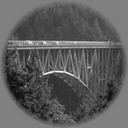
\includegraphics[scale = .52]{img1.png} & \hspace{1in} & 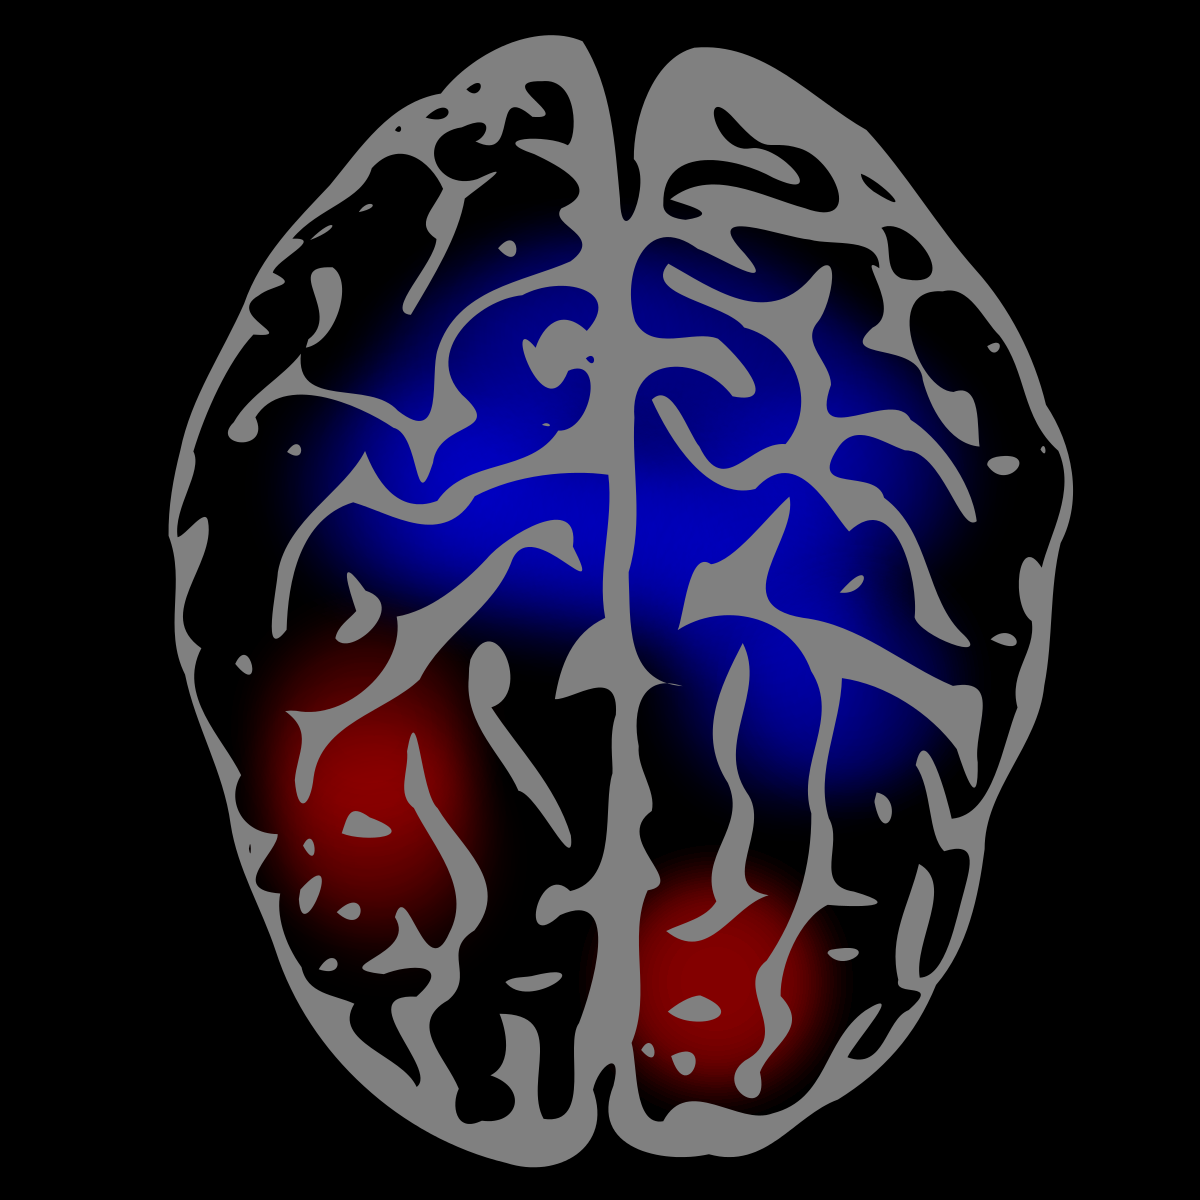
\includegraphics[scale = 0.07]{brain1.png} \\ \hline
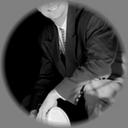
\includegraphics[scale = .52]{img2.png} & \hspace{1in} & 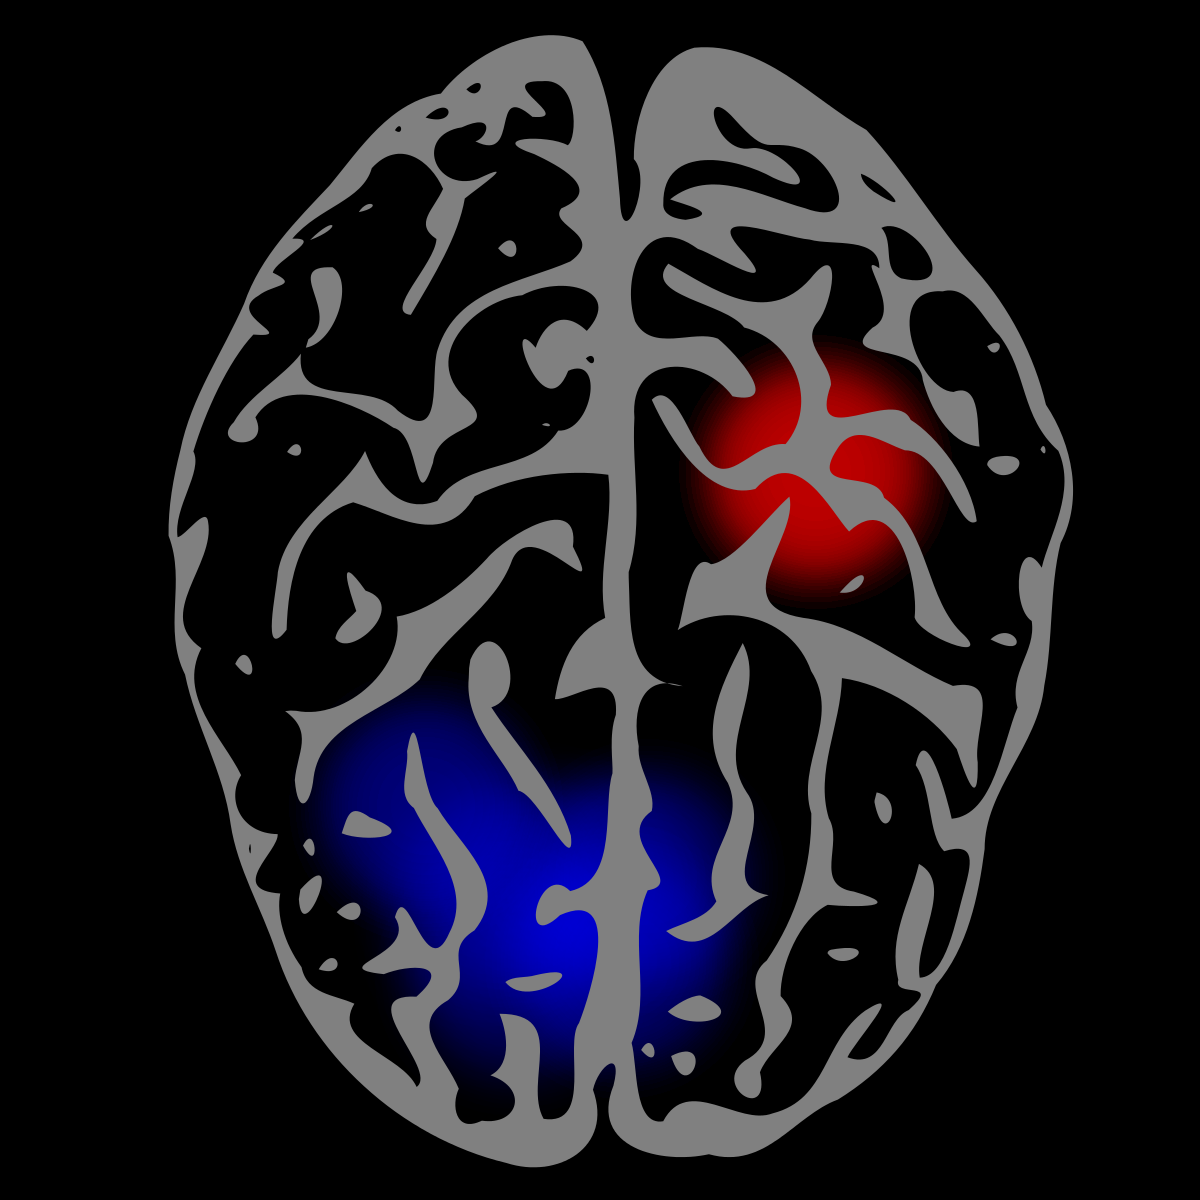
\includegraphics[scale = 0.07]{brain2.png} \\ \hline
\hspace{1in} & \hspace{1in} & \hspace{1in}
\end{tabular}
\end{center}
\end{frame}

\begin{frame}
\frametitle{Functional MRI}
\begin{center}
\begin{tabular}{ccc}
\hline
Stimuli $x$ & & Response $y$\\ \hline
$\begin{pmatrix}1.0 \\ 0 \\ 3.0 \\ 0\\ -1.2\end{pmatrix}$ & \hspace{1in} & $\begin{pmatrix}1.2 \\ 0 \\ -1.8\\ -1.2\end{pmatrix}$ \\ \hline
$\begin{pmatrix}0 \\ -2.2 \\ -3.1 \\ 4.5\\ 0\end{pmatrix}$ & \hspace{1in} & $\begin{pmatrix}-1.2 \\ -1.9\\ 0.5\\ 0.6\end{pmatrix}$ \\ \hline
\hspace{1in} & \hspace{1in} & \hspace{1in}
\end{tabular}
\end{center}
\end{frame}

\begin{frame}
\frametitle{Encoding vs Decoding}
\begin{itemize}
\item Encoding: predict $y$ from $x$.
\item Decoding: reconstruct $x$ from $y$ (mind-reading).
\begin{itemize}
\item Classification: label response $y$ by a class from the training data
\item Identification: label response $y$ by a class \emph{outside} of the training data
\item Reconstruction: infer $x$ from $y$
\end{itemize}
\end{itemize}
\end{frame}

\begin{frame}
\frametitle{Classification}
\begin{center}
Training Data
\\
\begin{tabular}{ccc||ccc}
\hline
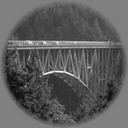
\includegraphics[scale = .26]{img1.png} & \hspace{0.2in} & 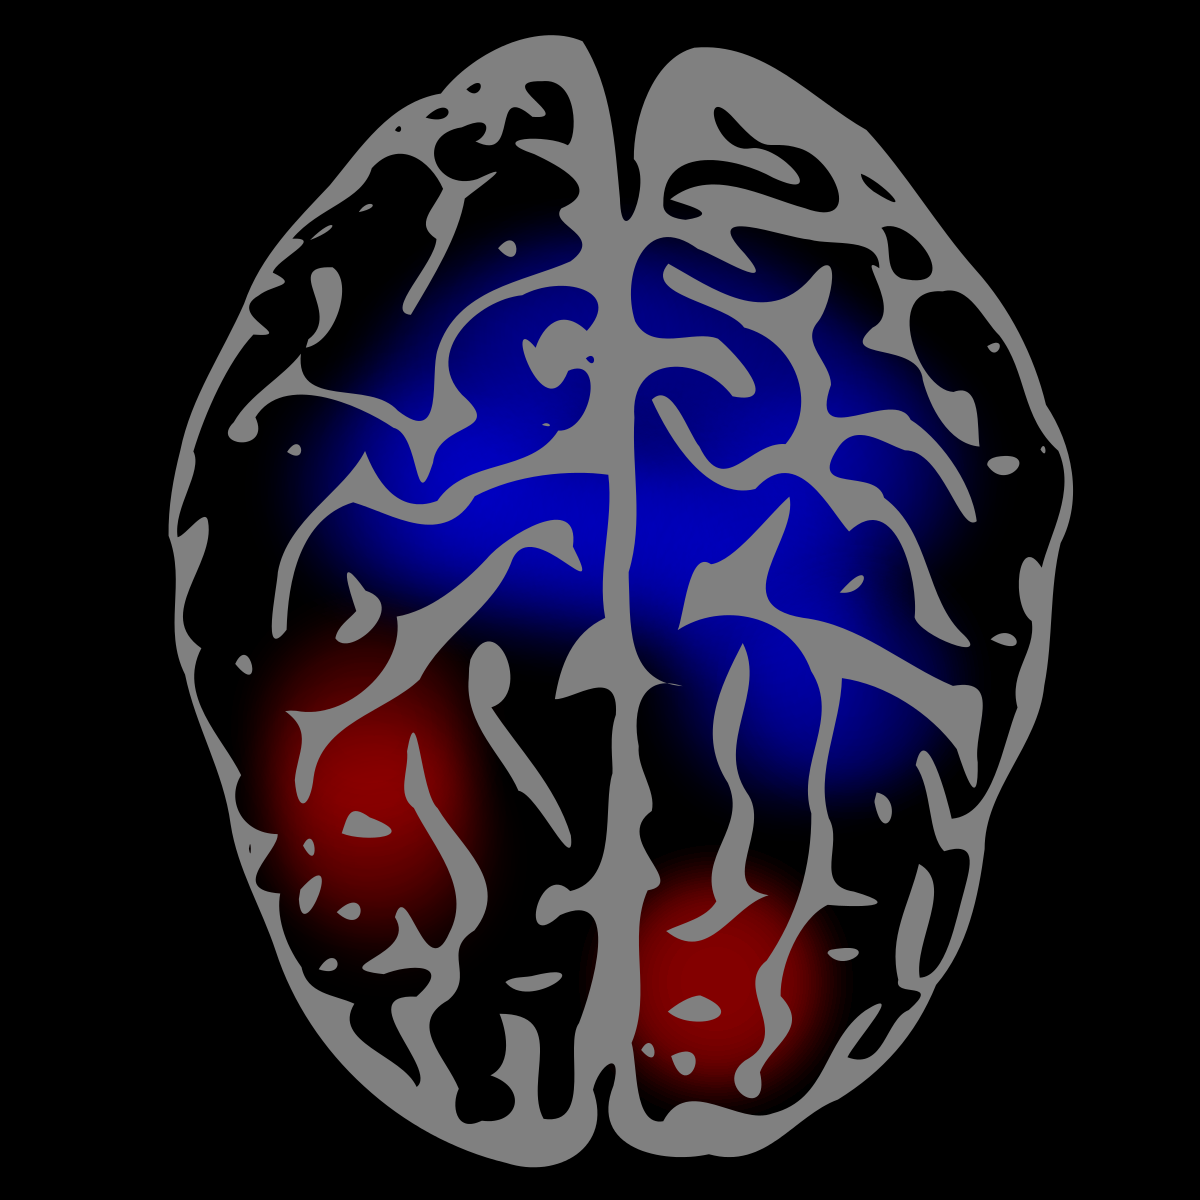
\includegraphics[scale = 0.035]{brain1.png} &
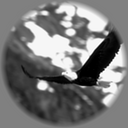
\includegraphics[scale = .26]{img3.png} & \hspace{0.2in} & 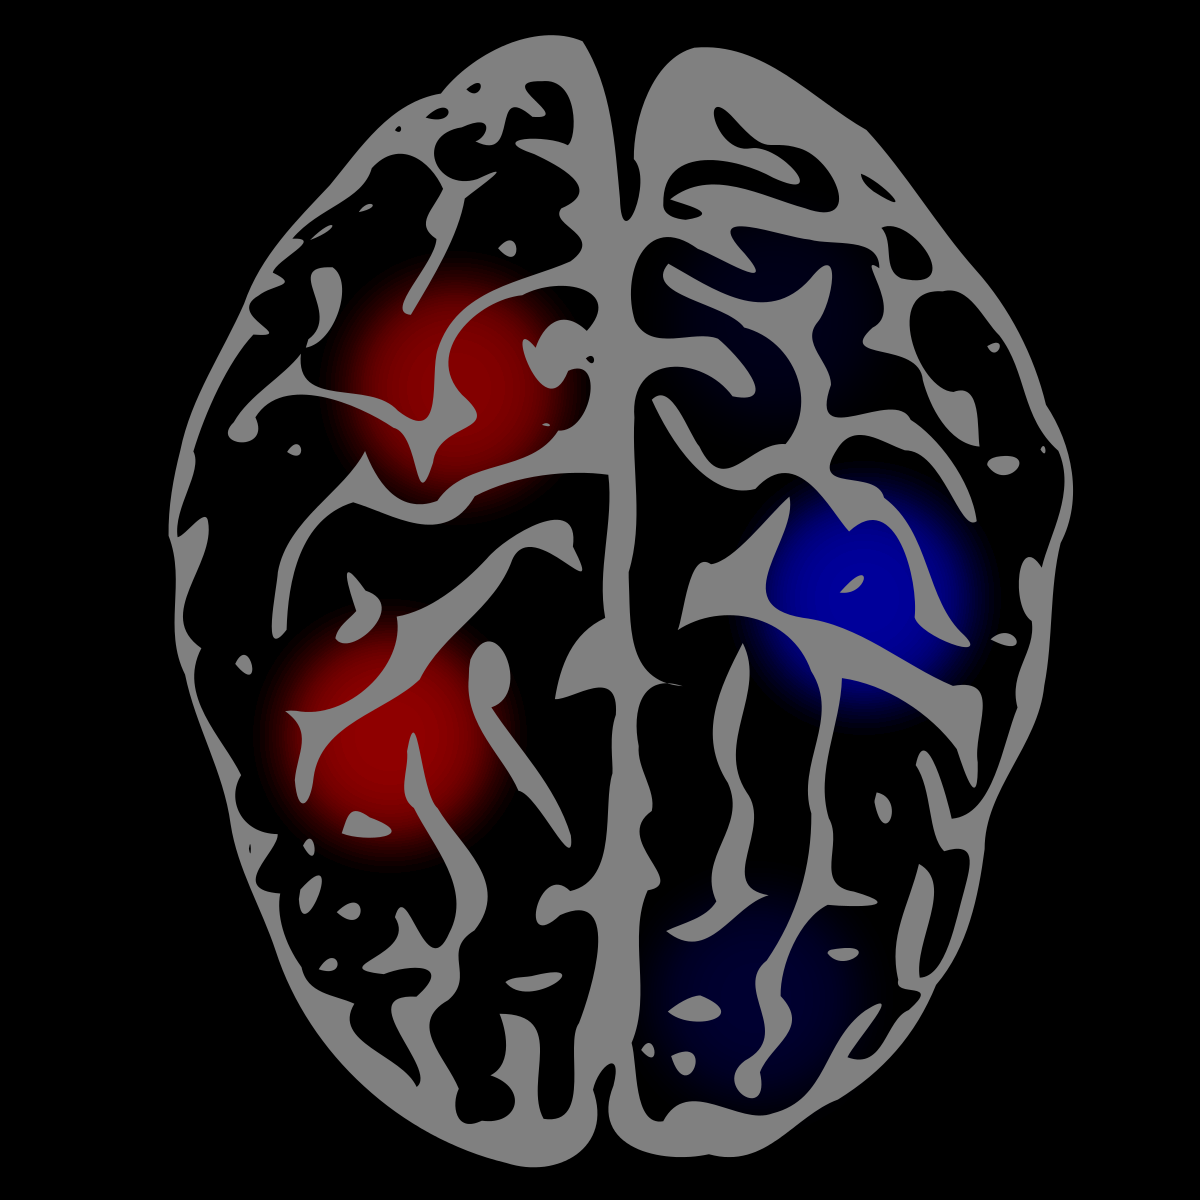
\includegraphics[scale = 0.035]{brain3.png} \\ \hline
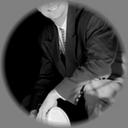
\includegraphics[scale = .26]{img2.png} & \hspace{0.2in} & 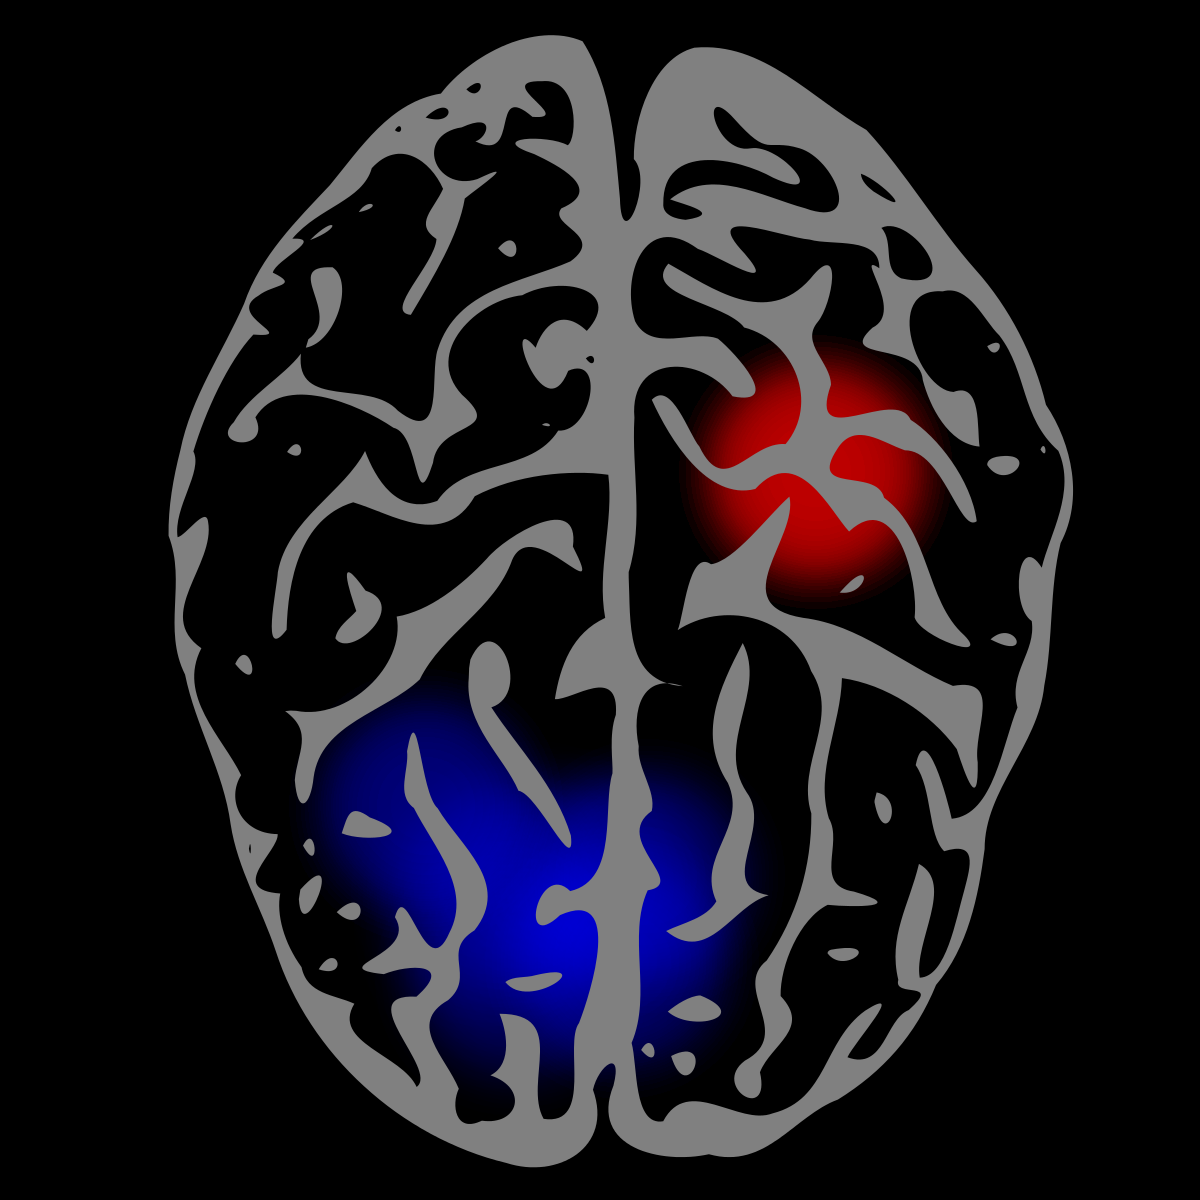
\includegraphics[scale = 0.035]{brain2.png} &
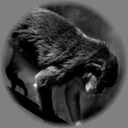
\includegraphics[scale = .26]{img4.png} & \hspace{0.2in} & 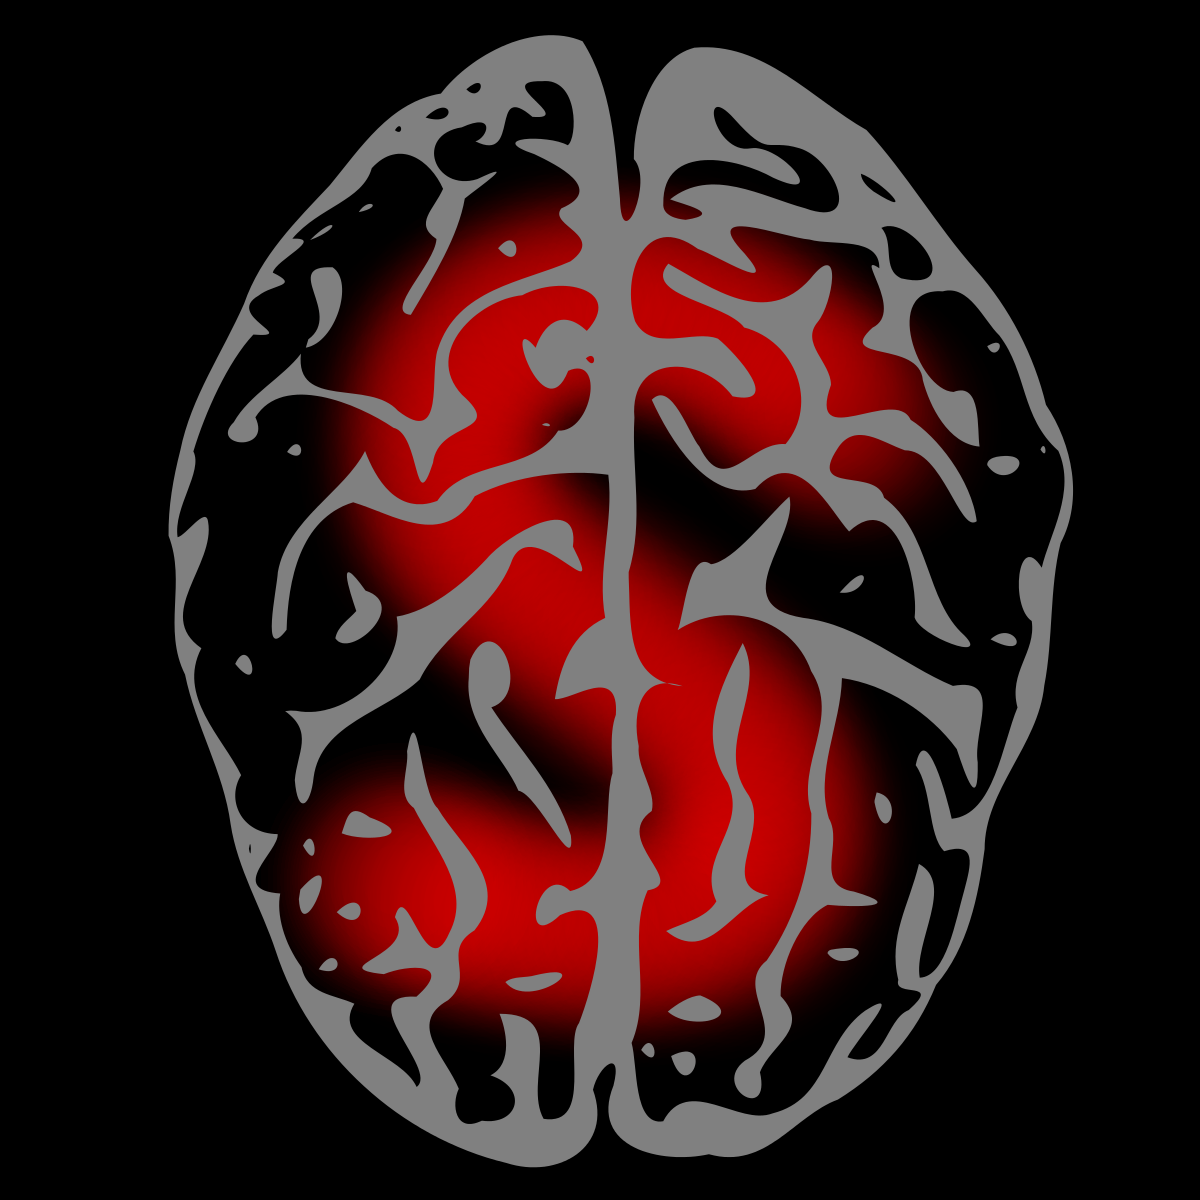
\includegraphics[scale = 0.035]{brain5.png} \\ \hline
\end{tabular}\\
\vspace{0.1in}
Test Data \\
\begin{tabular}{c|c|cccc}
\hline
 & & ? & ? & ? & ? \\
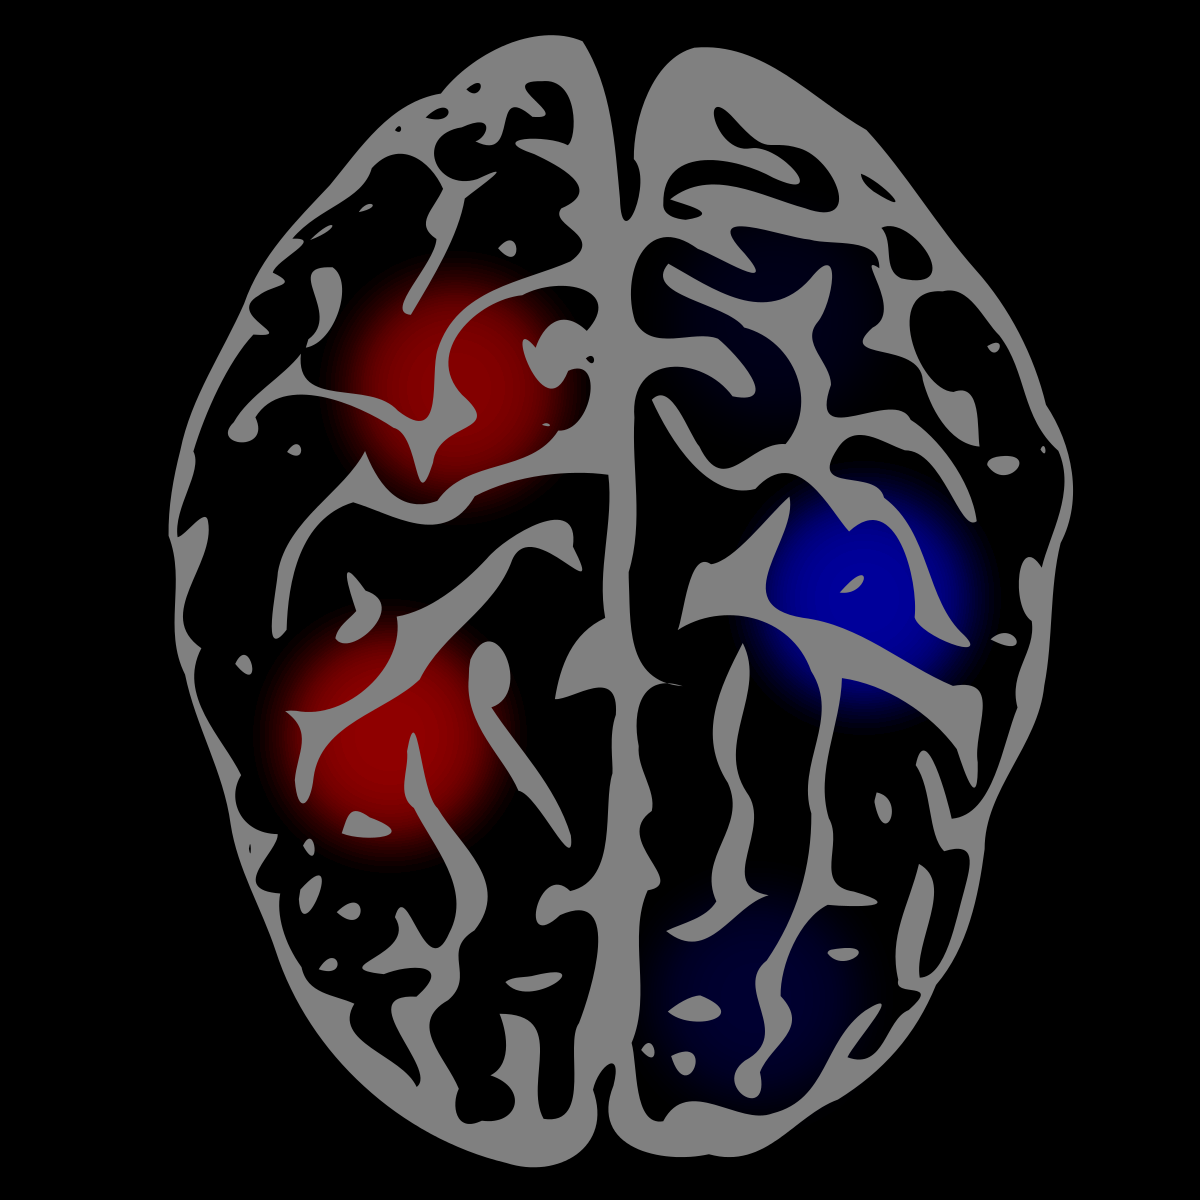
\includegraphics[scale = 0.035]{brain3.png} & \hspace{0.5in} 
& 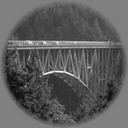
\includegraphics[scale = .26]{img1.png}
& 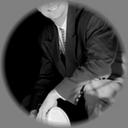
\includegraphics[scale = .26]{img2.png}
& 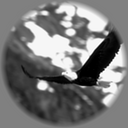
\includegraphics[scale = .26]{img3.png}
& 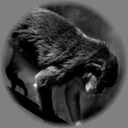
\includegraphics[scale = .26]{img4.png}\\
\hline
 & & ? & ? & ? & ? \\
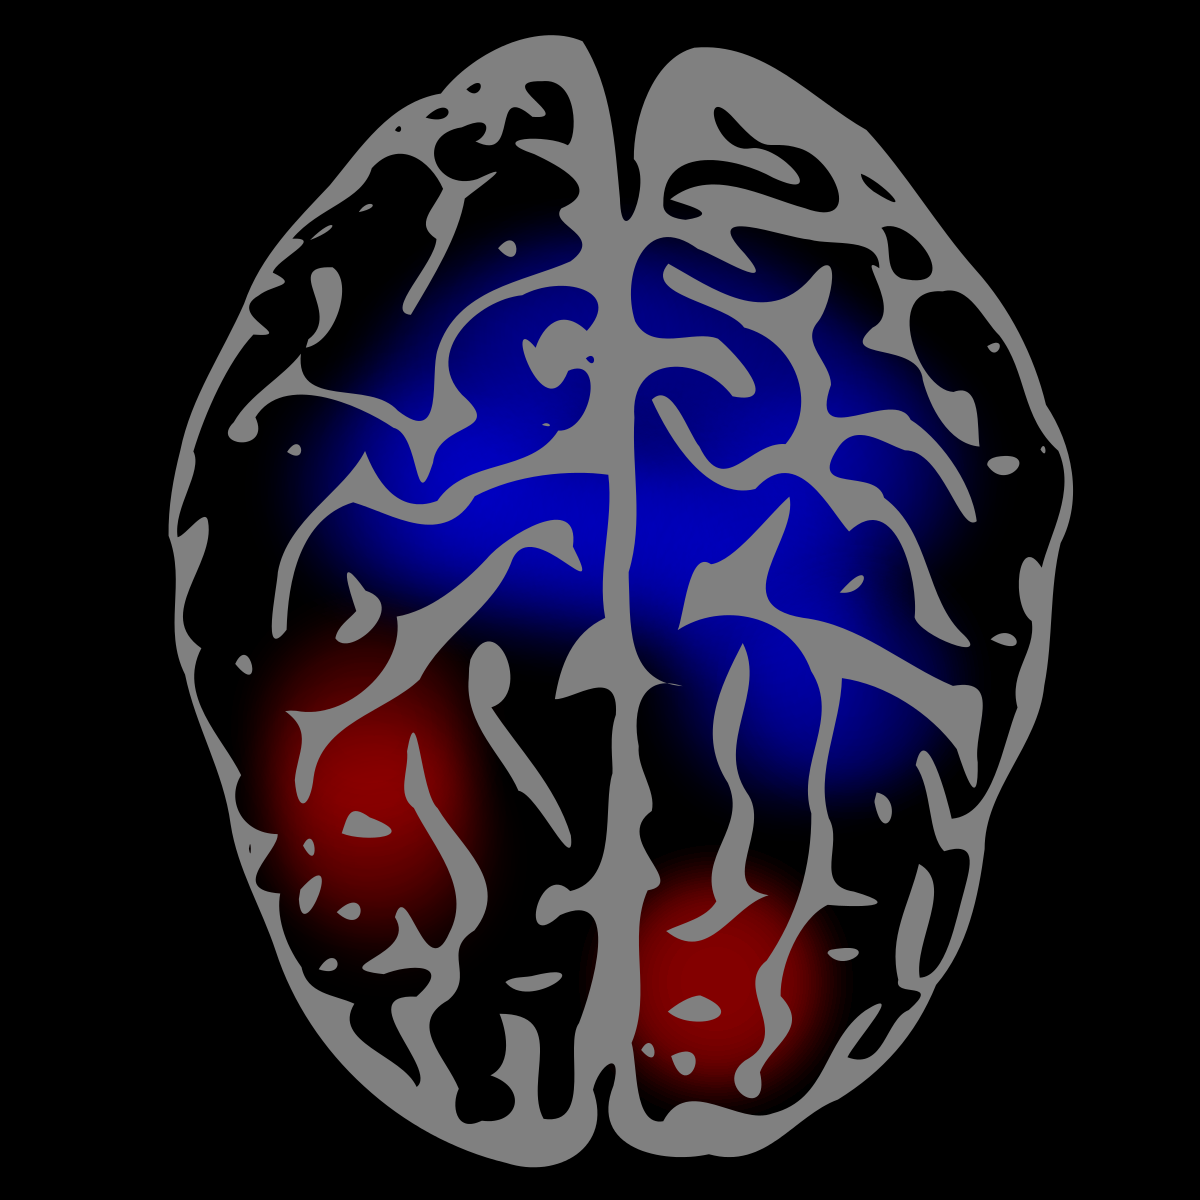
\includegraphics[scale = 0.035]{brain1.png} & \hspace{0.5in} 
& 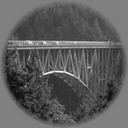
\includegraphics[scale = .26]{img1.png}
& 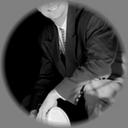
\includegraphics[scale = .26]{img2.png}
& 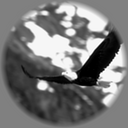
\includegraphics[scale = .26]{img3.png}
& 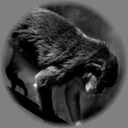
\includegraphics[scale = .26]{img4.png}\\
\hline
\end{tabular}
\end{center}
\end{frame}


\begin{frame}
\frametitle{Classification}
\begin{center}
Training Data
\\
\begin{tabular}{ccc||ccc}
\hline
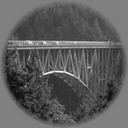
\includegraphics[scale = .26]{img1.png} & \hspace{0.2in} & 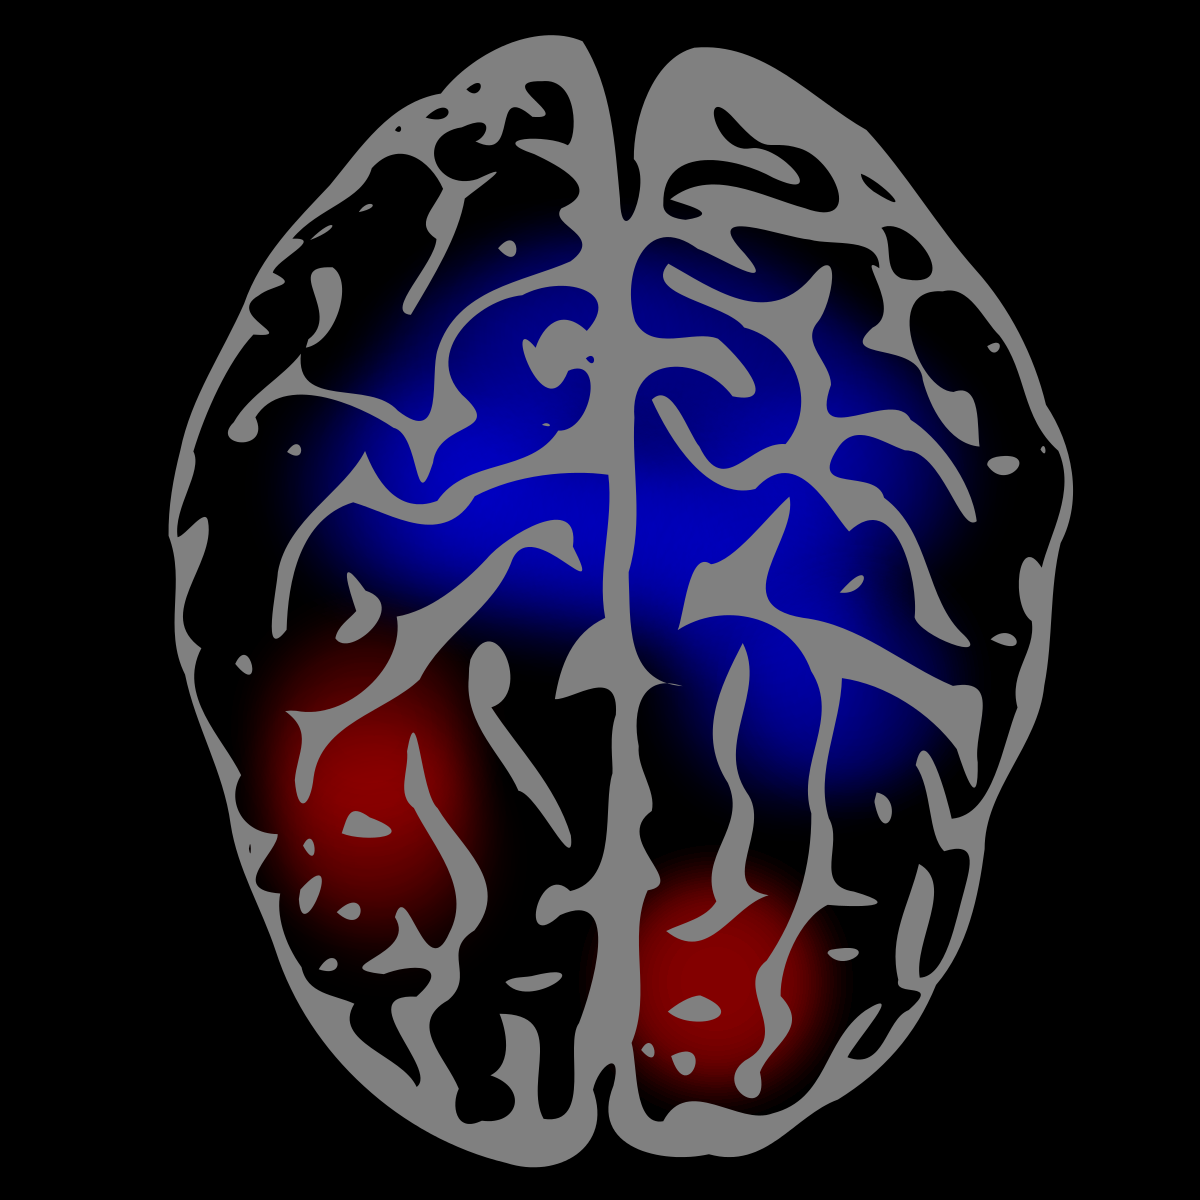
\includegraphics[scale = 0.035]{brain1.png} &
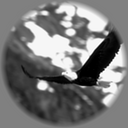
\includegraphics[scale = .26]{img3.png} & \hspace{0.2in} & 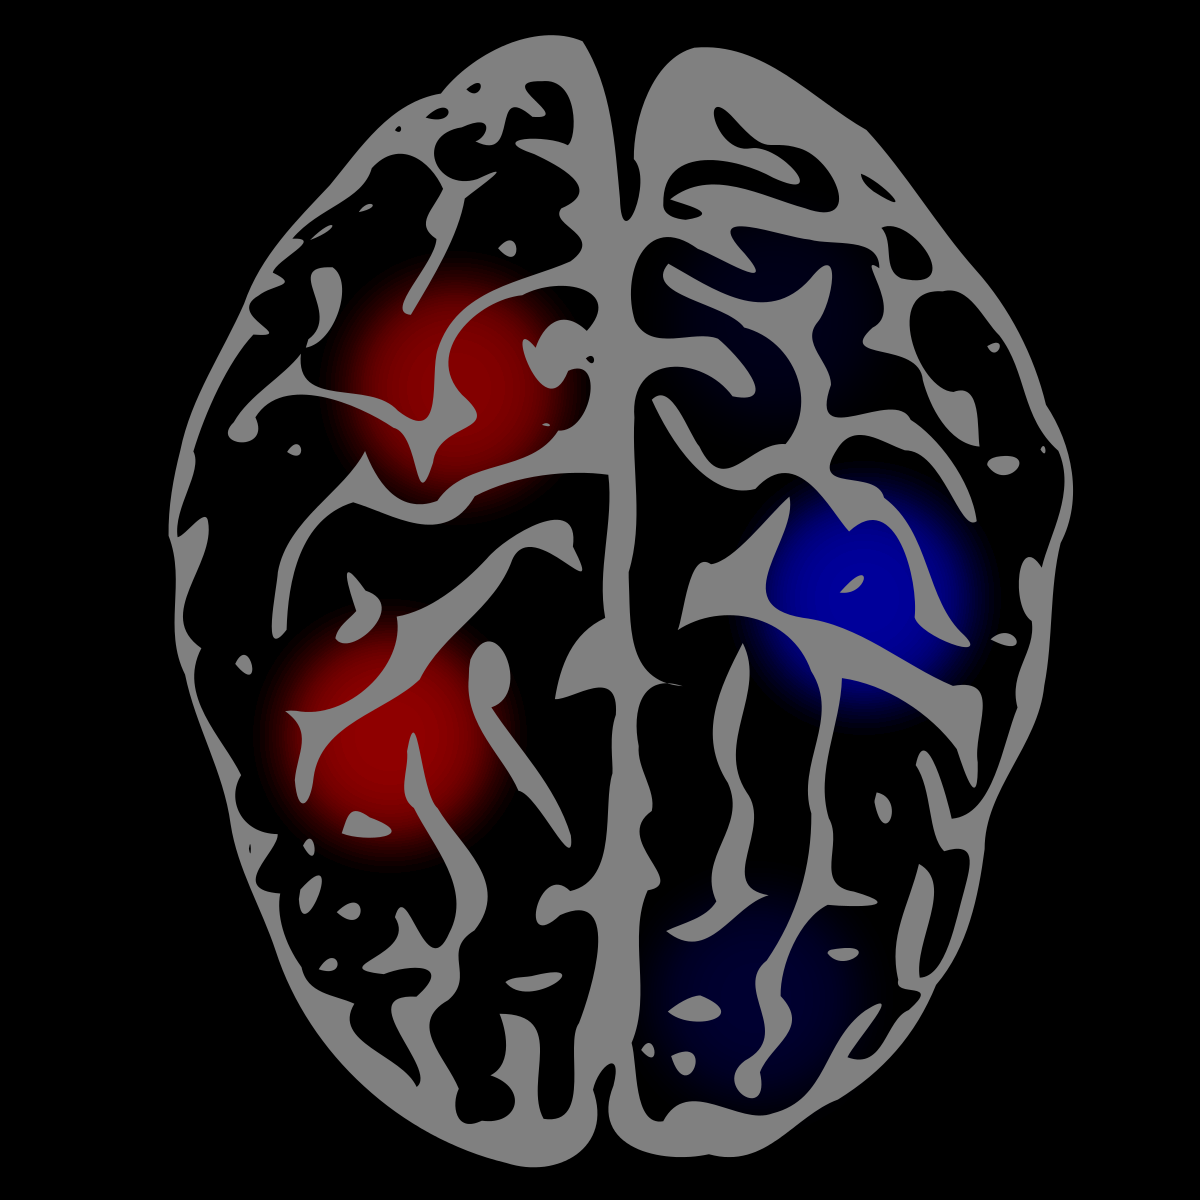
\includegraphics[scale = 0.035]{brain3.png} \\ \hline
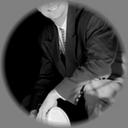
\includegraphics[scale = .26]{img2.png} & \hspace{0.2in} & 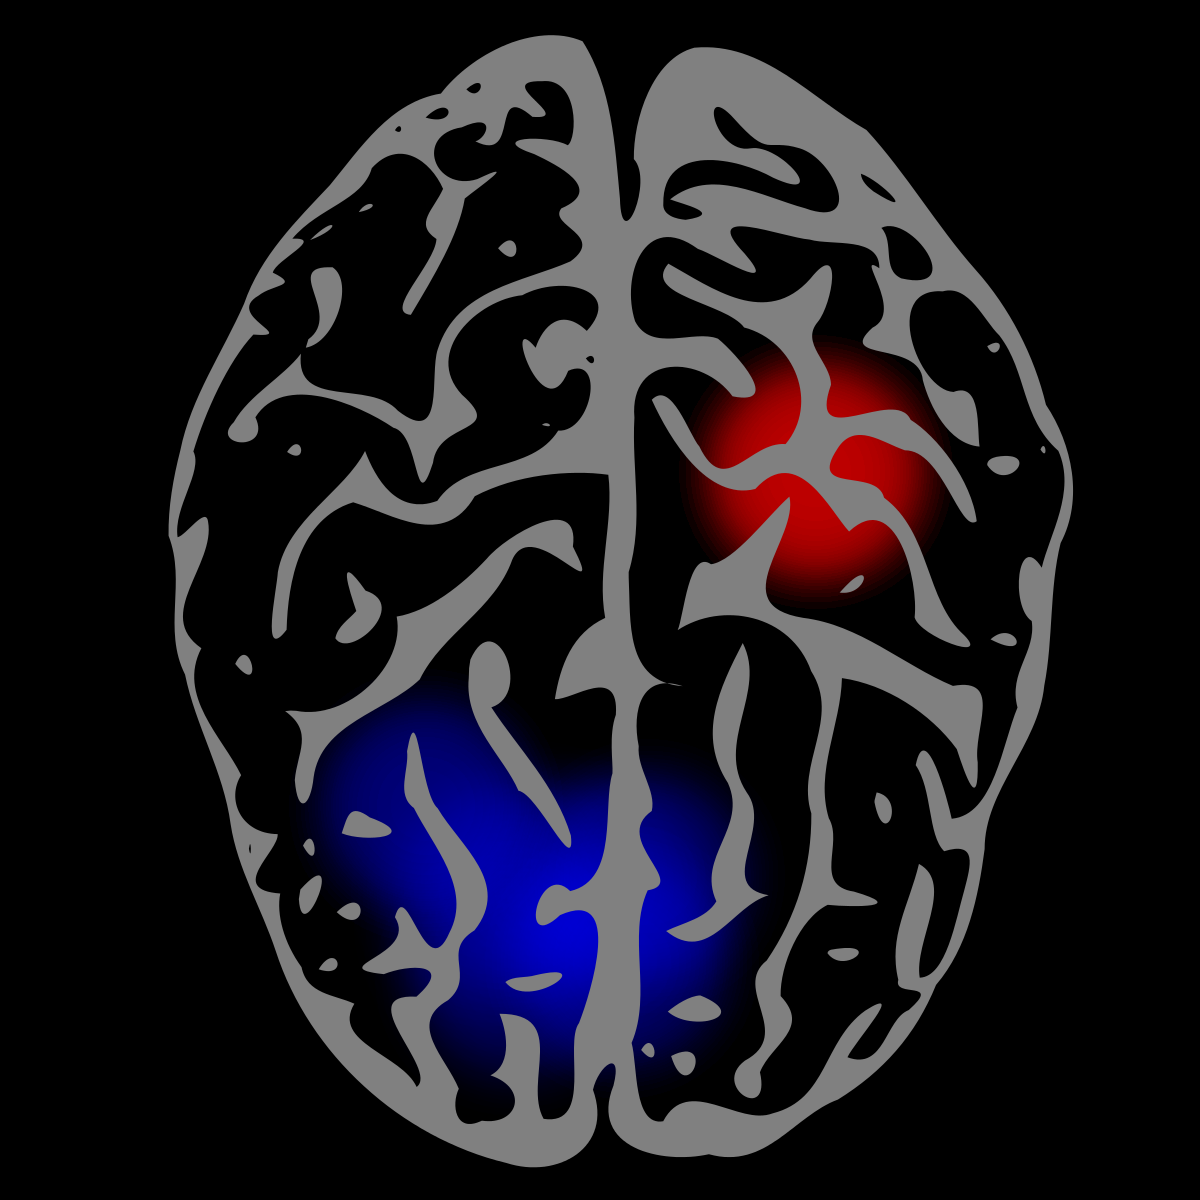
\includegraphics[scale = 0.035]{brain2.png} &
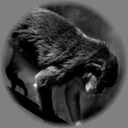
\includegraphics[scale = .26]{img4.png} & \hspace{0.2in} & 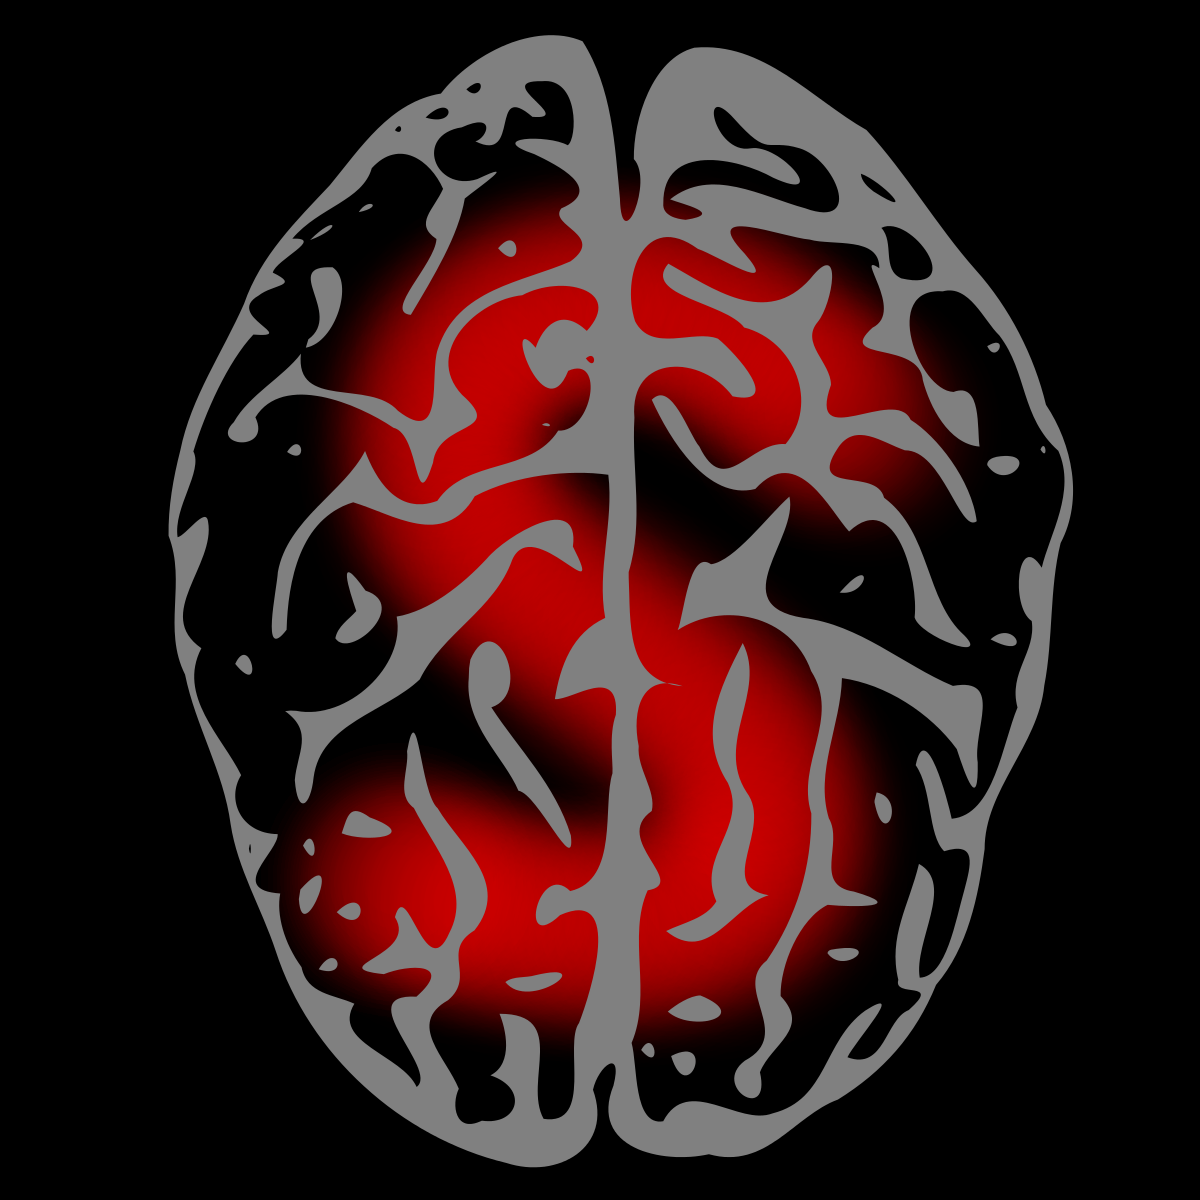
\includegraphics[scale = 0.035]{brain5.png} \\ \hline
\end{tabular}\\
\vspace{0.1in}
Test Data \\
\begin{tabular}{c|c|cccc}
\hline
 & & \xmark & \xmark & \cmark & \xmark \\
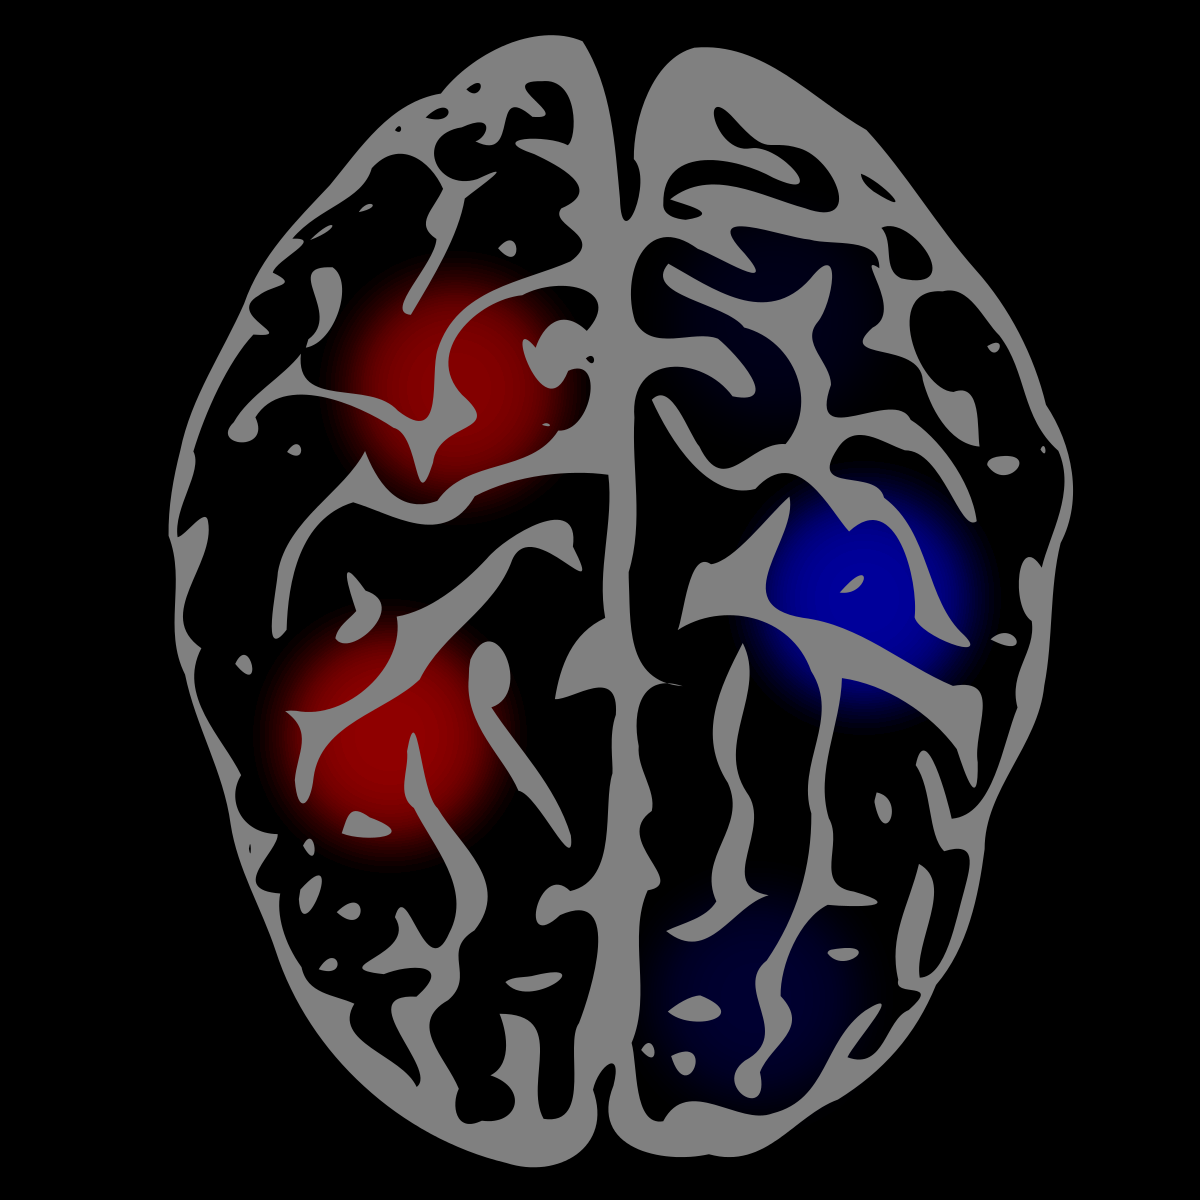
\includegraphics[scale = 0.035]{brain3.png} & \hspace{0.5in} 
& 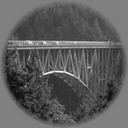
\includegraphics[scale = .26]{img1.png}
& 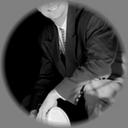
\includegraphics[scale = .26]{img2.png}
& 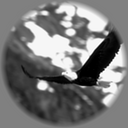
\includegraphics[scale = .26]{img3.png}
& 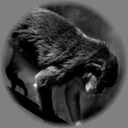
\includegraphics[scale = .26]{img4.png}\\
\hline
 & & \cmark & \xmark & \xmark & \xmark \\
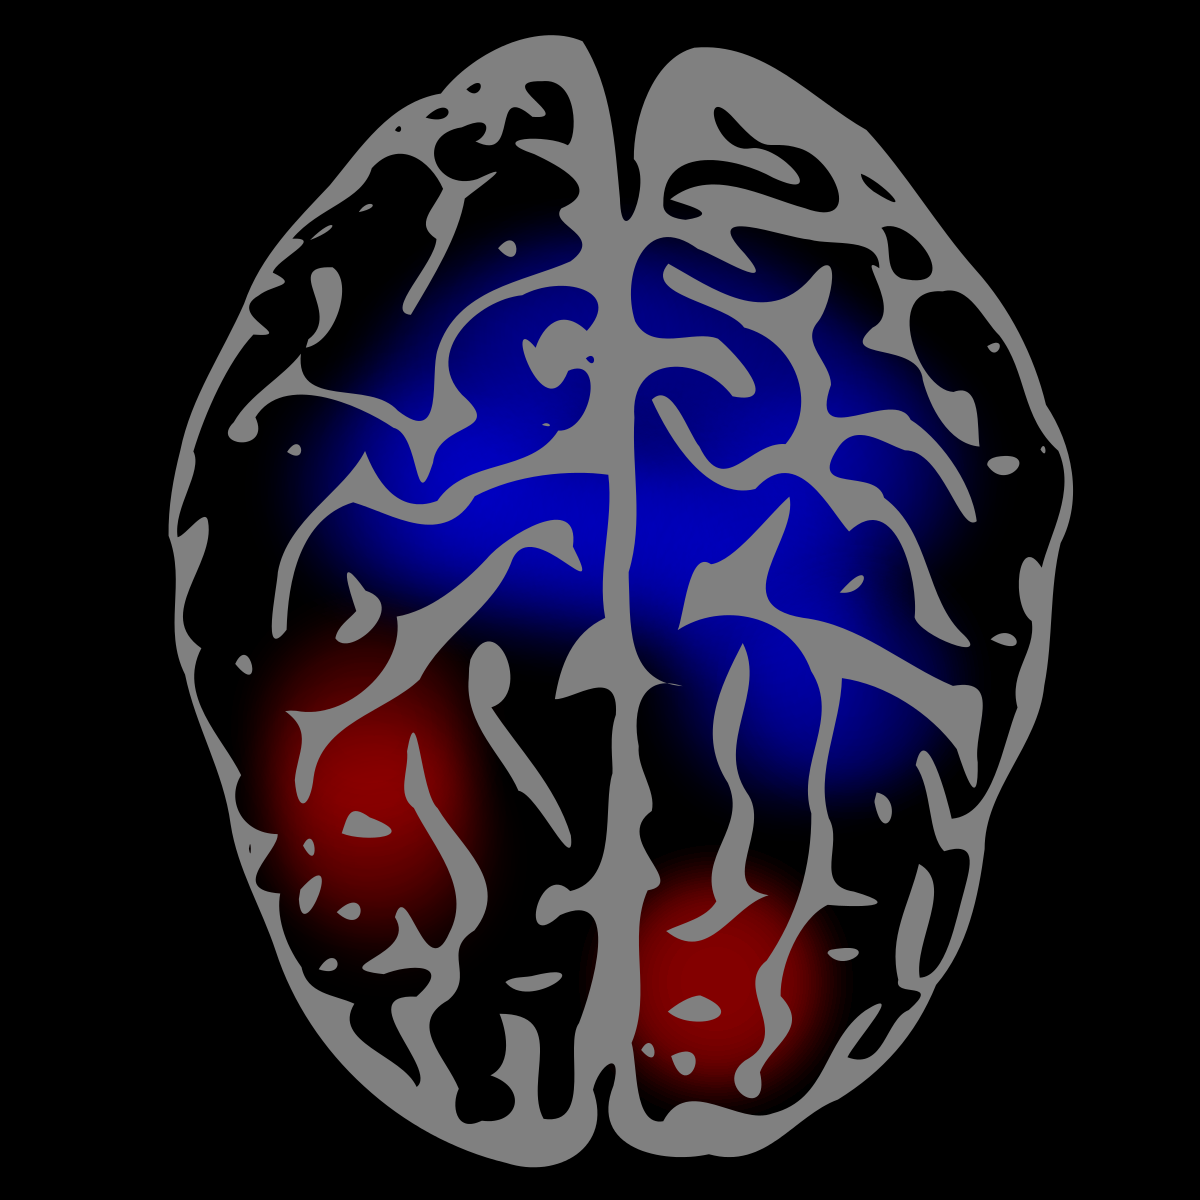
\includegraphics[scale = 0.035]{brain1.png} & \hspace{0.5in} 
& 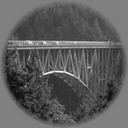
\includegraphics[scale = .26]{img1.png}
& 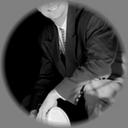
\includegraphics[scale = .26]{img2.png}
& 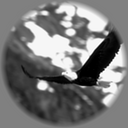
\includegraphics[scale = .26]{img3.png}
& 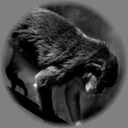
\includegraphics[scale = .26]{img4.png}\\
\hline
\end{tabular}
\end{center}
\end{frame}

\begin{frame}
\frametitle{Identification}
\begin{center}
Training Data
\\
\begin{tabular}{ccc||ccc}
\hline
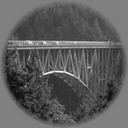
\includegraphics[scale = .26]{img1.png} & \hspace{0.2in} & 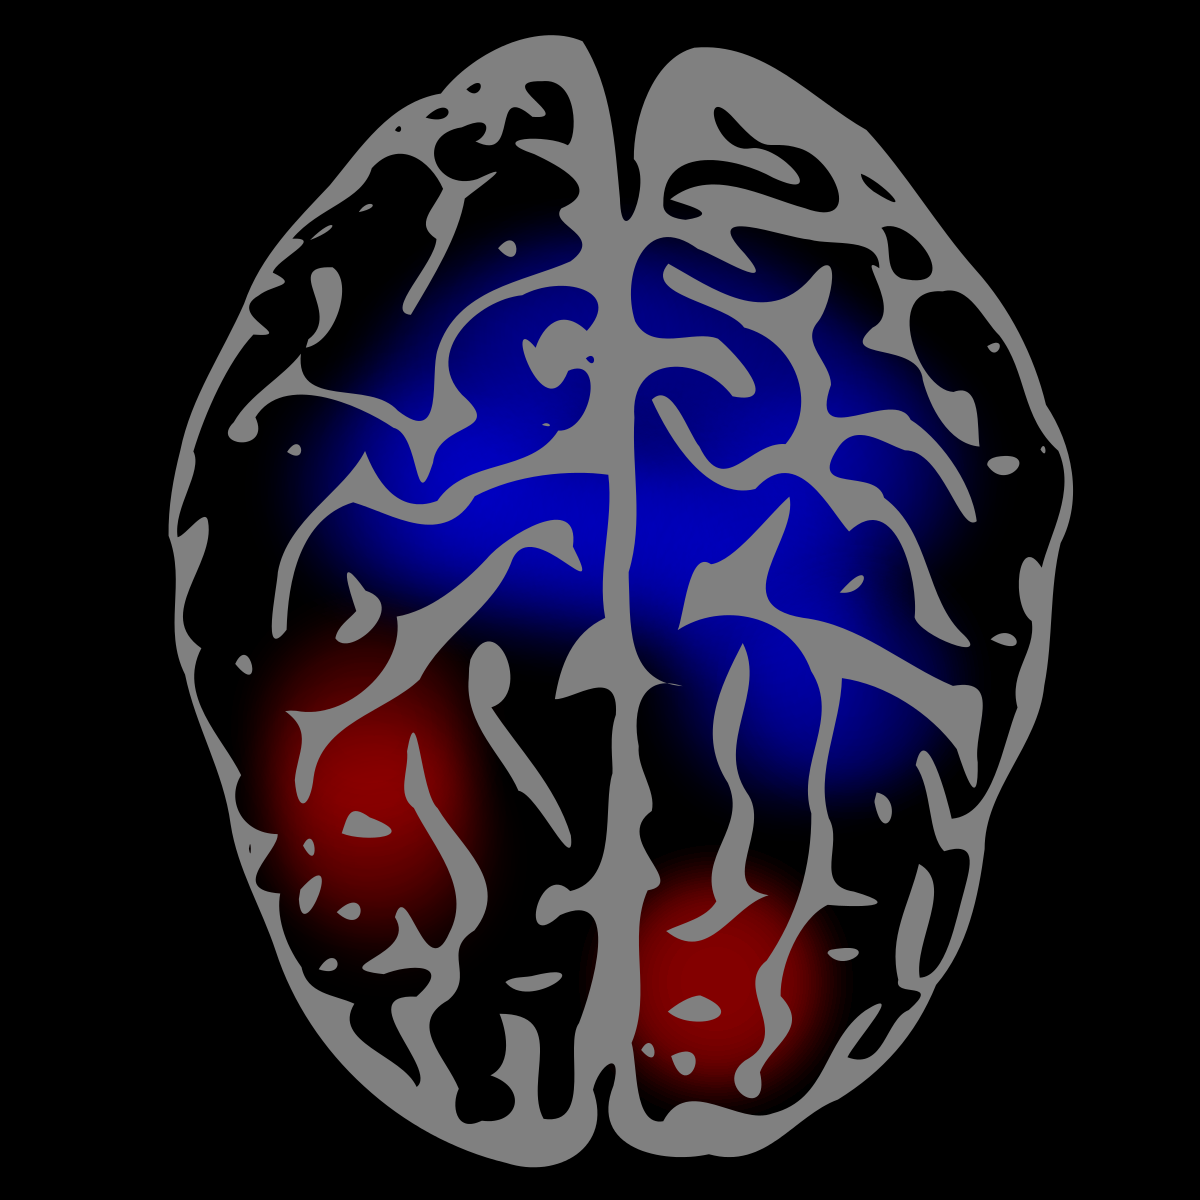
\includegraphics[scale = 0.035]{brain1.png} &
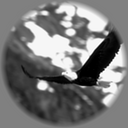
\includegraphics[scale = .26]{img3.png} & \hspace{0.2in} & 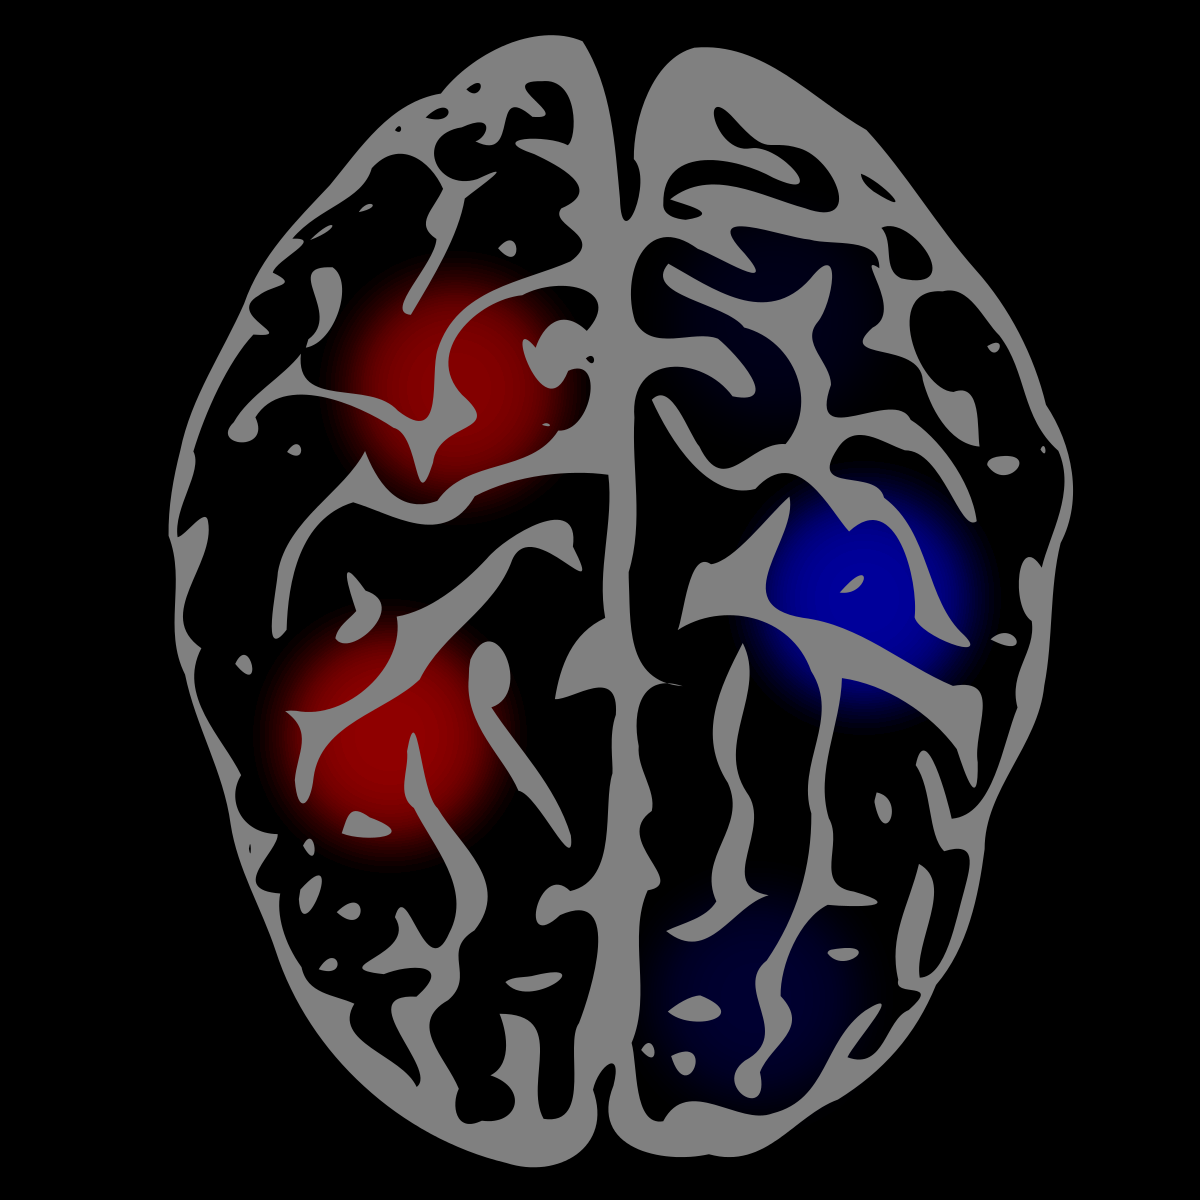
\includegraphics[scale = 0.035]{brain3.png} \\ \hline
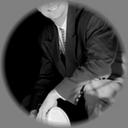
\includegraphics[scale = .26]{img2.png} & \hspace{0.2in} & 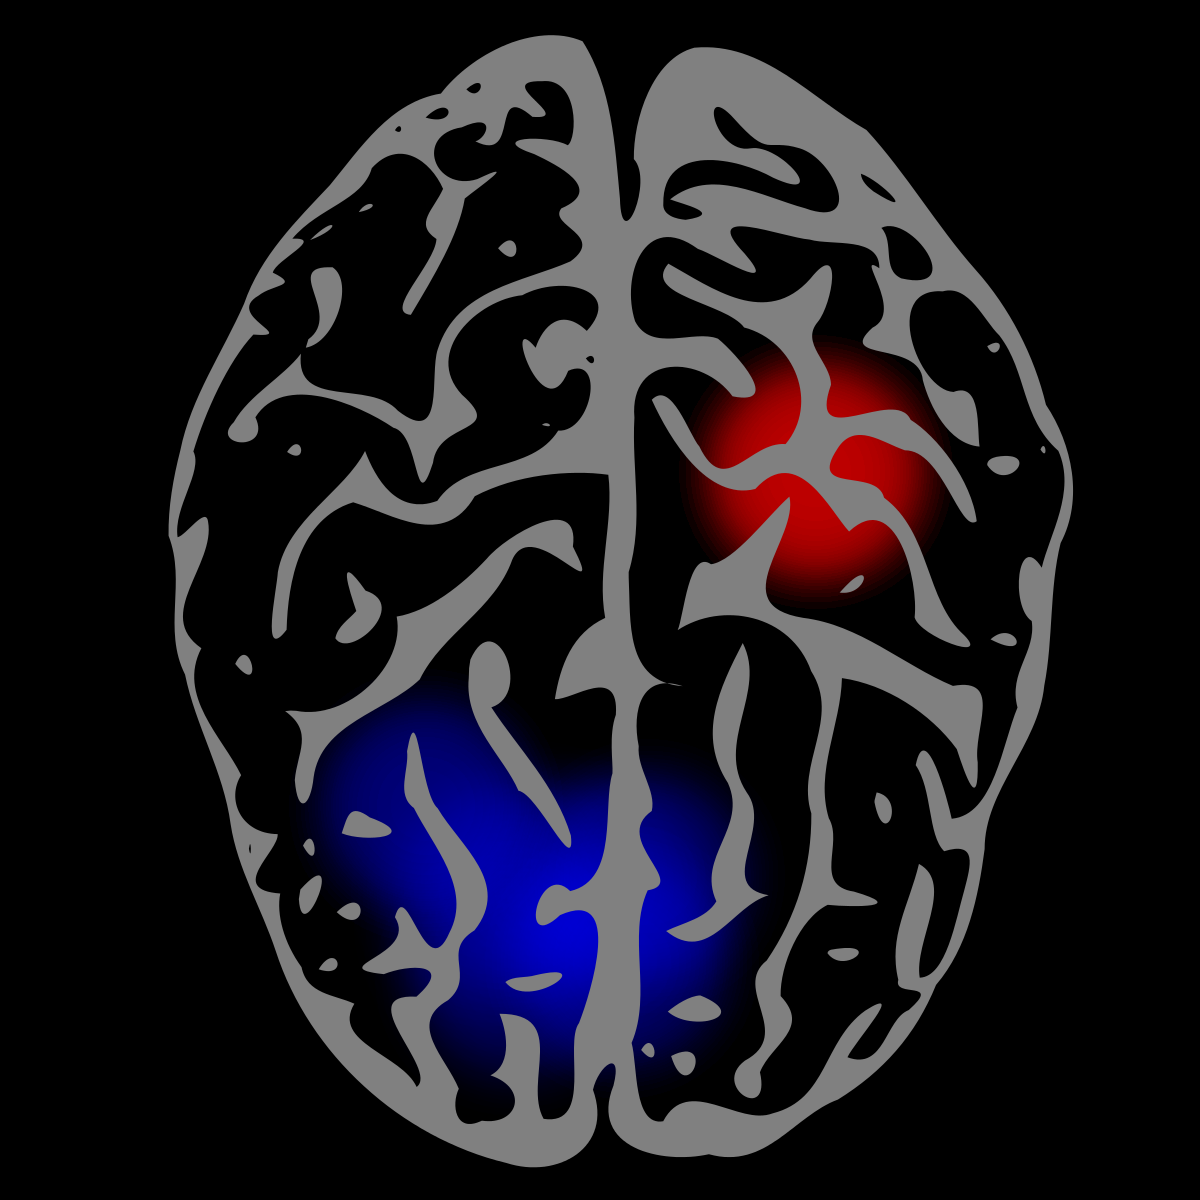
\includegraphics[scale = 0.035]{brain2.png} &
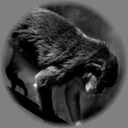
\includegraphics[scale = .26]{img4.png} & \hspace{0.2in} & 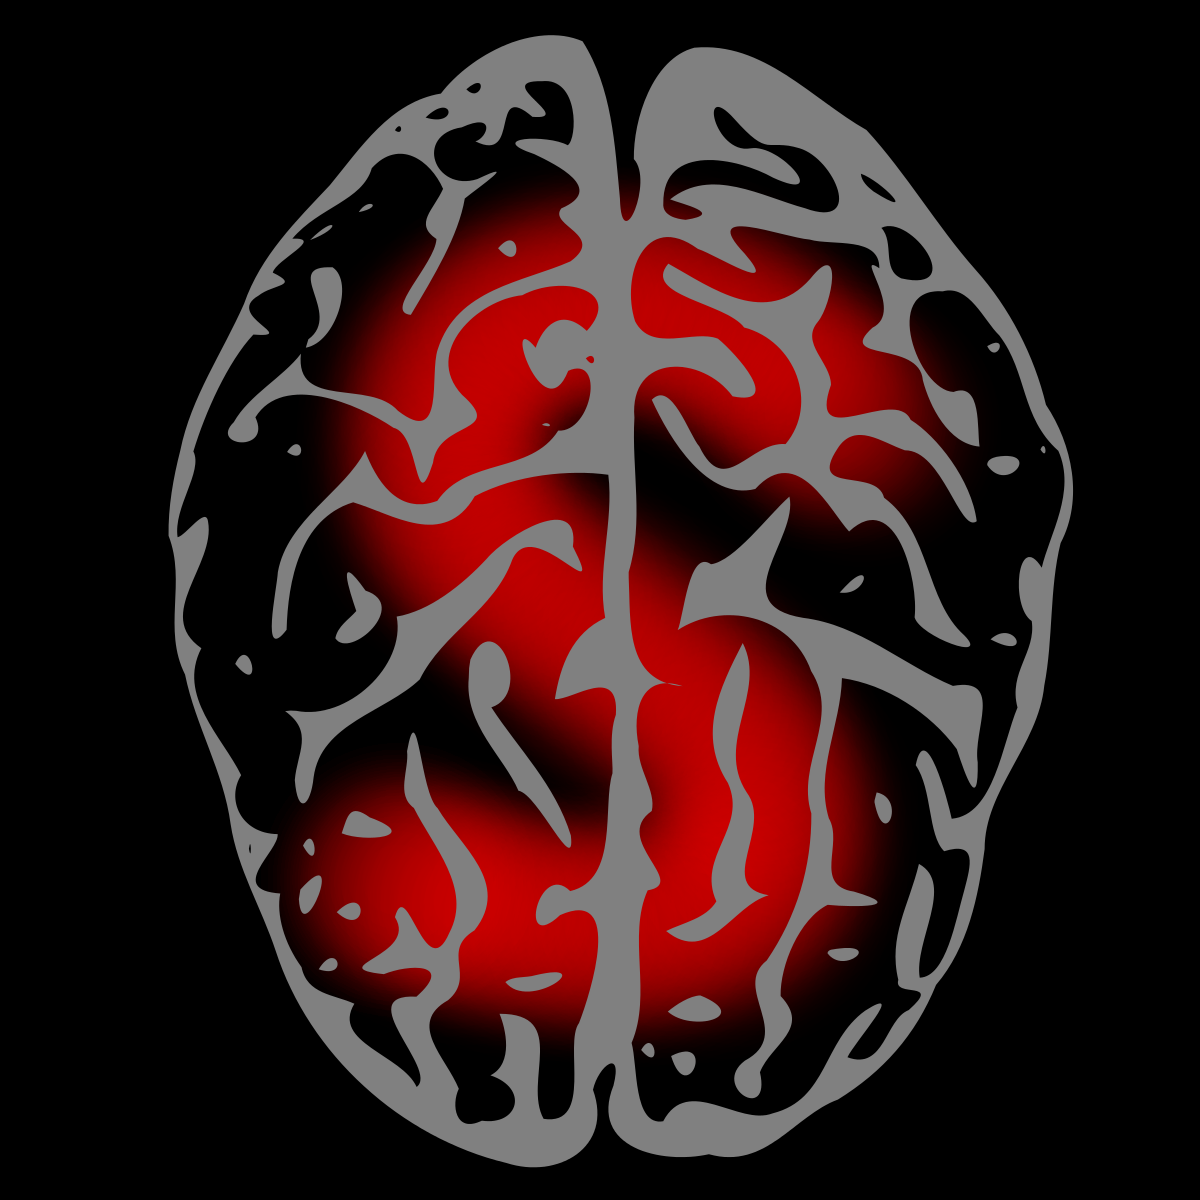
\includegraphics[scale = 0.035]{brain5.png} \\ \hline
\end{tabular}\\
\vspace{0.1in}
Test Data \emph{(new images!)} \\
\begin{tabular}{c|c|cccc}
\hline
 & & ? & ? & ? & ? \\
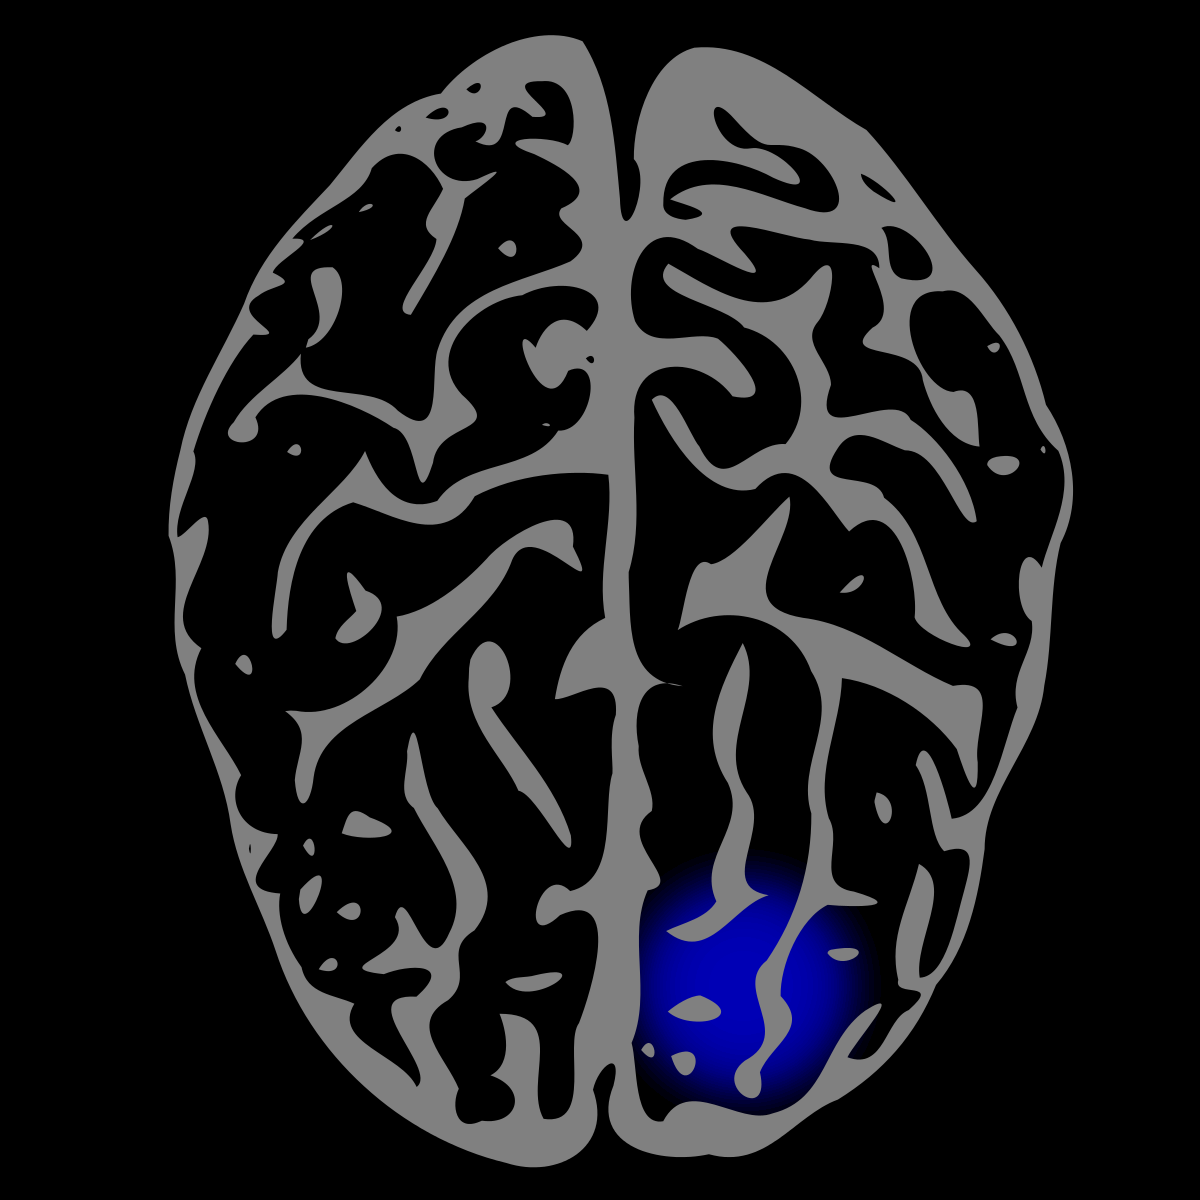
\includegraphics[scale = 0.035]{brain7.png} & \hspace{0.5in} 
& 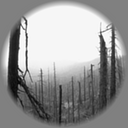
\includegraphics[scale = .26]{img5.png}
& \includegraphics[scale = .26]{img6.png}
& \includegraphics[scale = .26]{img7.png}
& \includegraphics[scale = .26]{img8.png}\\
\hline
 & & ? & ? & ? & ? \\
\includegraphics[scale = 0.035]{brain8.png} & \hspace{0.5in} 
& \includegraphics[scale = .26]{img5.png}
& \includegraphics[scale = .26]{img6.png}
& \includegraphics[scale = .26]{img7.png}
& \includegraphics[scale = .26]{img8.png}\\
\hline
\end{tabular}
\end{center}
\end{frame}

\begin{frame}
\begin{center}
\includegraphics[scale = 0.4]{kay00.png}
\includegraphics[scale = 0.4]{kay01.png}
\end{center}
\end{frame}

\begin{frame}
\frametitle{Reconstruction}
\begin{center}
Training Data
\\
\begin{tabular}{ccc||ccc}
\hline
\includegraphics[scale = .26]{img1.png} & \hspace{0.2in} & \includegraphics[scale = 0.035]{brain1.png} &
\includegraphics[scale = .26]{img3.png} & \hspace{0.2in} & \includegraphics[scale = 0.035]{brain3.png} \\ \hline
\includegraphics[scale = .26]{img2.png} & \hspace{0.2in} & \includegraphics[scale = 0.035]{brain2.png} &
\includegraphics[scale = .26]{img4.png} & \hspace{0.2in} & \includegraphics[scale = 0.035]{brain5.png} \\ \hline
\end{tabular}\\
\vspace{0.1in}
Test Data \emph{(new images!)} \\
\begin{tabular}{c||c||c|c}
\hline

Stimulus & Response & Standard basis & Gabor basis\\
\includegraphics[scale = 0.22]{i11.png} 
& \includegraphics[scale = 0.035]{brain7.png} 
& \includegraphics[scale = .22]{i12.png}
& \includegraphics[scale = .22]{i13.png}\\ \hline
\includegraphics[scale = 0.22]{i21.png} 
& \includegraphics[scale = 0.035]{brain8.png} 
& \includegraphics[scale = .22]{i22.png}
& \includegraphics[scale = .22]{i23.png}\\ \hline
\end{tabular}
\end{center}
\end{frame}

\begin{frame}
\frametitle{Classification vs Identification vs Reconstruction}
\begin{itemize}
\item Classification is easy: doesn't require domain-specific model
\item Identification and reconstruction both require a model relating image features to responses
\end{itemize}
\begin{center}
\emph{Difficulty of Identification vs Reconstruction}
\begin{tabular}{|c|c|c|}
\hline
&  High dimensions & Number of candidate stimuli \\ \hline
Identification & Neutral & Hard \\ \hline
Reconstruction & Hard & Easy \\ \hline
\end{tabular}
\end{center}
\end{frame}

\begin{frame}
\frametitle{Motivating questions}
\begin{itemize}
\item
Under what conditions would it be possible to get performance on
reconstruction or identification?
\item
How can we develop methods which achieve better performance on these
tasks?
\item
Can we interpret the performance metric (prediction error,
misclassification error) of a model to draw scientific conclusions?
(E.g. which features are important, information content of fMRI scan.)
\end{itemize}
\end{frame}



\begin{frame}
\frametitle{Classification vs Identification vs Reconstruction}
\begin{center}
\emph{Supervised learning problems}
\begin{tabular}{|c|c|c|}
\hline
 & Misclassification Rate & Prediction error \\ \hline
No covariates & Classification & (nothing to predict) \\ \hline
Covariates ($x$) & Identification & Regression \\ \hline
\end{tabular}
\end{center}
\begin{itemize}
\item Reconstruction is regression $ x \sim y$
\item Does there already exist statistical theory for identification?
\item Next: a toy model for identification
\end{itemize}
\end{frame}

\section{Theory}

\frame{\sectionpage}

\begin{frame}
\frametitle{The problem of identification}
\emph{Training data.}
\begin{itemize}
\item
Given training classes $S_{\text{train}} = \{\text{train:}1,\hdots,
\text{train:}k\}$ where each class $\text{train:}i$ has features
$x_{\text{train:}i}$.
\item
For $t = 1,\hdots, T_{\text{train}}$, choose class label
$z_{\text{train:} t} \in S_{\text{train}}$; sample a response
$y_{\text{train:} t}$ from that class.
\end{itemize}
\emph{Test data.}
\begin{itemize}
\item
Given test classes $S_{\text{test}} = \{\text{test:}1,\hdots,
\text{test:}\ell\}$ with features $\{x_{\text{test:} 1}, \hdots,
x_{\text{test:} \ell}\}$
\item
Task: for $t = 1,\hdots, T_{\text{test}}$, label $y_{\text{test}: t}$
by class $\hat{z}_{\text{test:} t} \in S_{\text{train}}$; try to
minimize misclassification rate
\end{itemize}
\end{frame}

\begin{frame}
\frametitle{Additional assumptions}
\begin{itemize}
\item For a point $y$ from class with features $x$,
\[
y = f(x) + \epsilon
\]
where the noise $\epsilon$ is drawn from some distribution and $f$ is an unknown function
\item The features for the training and test classes are sampled iid from the same distribution $P$
\[x_{\text{train:} i} \sim P\]
\[x_{\text{train:} i} \sim P\]
\end{itemize}
\end{frame}

\begin{frame}
\frametitle{Toy example I}
\begin{center}
\includegraphics[scale = 0.3]{1d_0.pdf}
\end{center}
\begin{itemize}
\item Features $x$ are one-dimensional real numbers, as are responses
  $y$.  Parameter $\beta$ is also a real number.
\item Model is linear: $y \sim N(x\beta, \sigma^2_\epsilon)$
\end{itemize}
\end{frame}

\begin{frame}
\begin{center}
\includegraphics[scale = 0.4]{ti1.pdf}
\end{center}
Suppose we estimated $\hat{\beta}$ from training data.
\end{frame}

\begin{frame}
\begin{center}
\includegraphics[scale = 0.4]{ti2.pdf}
\end{center}
Generate features $x_{\text{test:} 1}, \hdots, x_{\text{test:} \ell}$ iid $N(0, \sigma^2_x)$.
\end{frame}

\begin{frame}
\begin{center}
\includegraphics[scale = 0.4]{ti3.pdf}
\end{center}
Hidden labels $z_{\text{test:} t}$ are iid uniform from $S_{\text{train}}$.\\
Generate $y_{\text{test:} t} \sim N(\beta x_{z_{\text{test:} t}}, \sigma^2_\epsilon)$
\end{frame}

\begin{frame}
\begin{center}
\includegraphics[scale = 0.4]{ti4.pdf}
\end{center}
Classify $\hat{y}_{\text{test:} t}$
\end{frame}

\begin{frame}
\begin{center}
\includegraphics[scale = 0.4]{ti5.pdf}
\end{center}
$\hat{\mu}_{\text{test:} i} = \hat{\beta} x_{\text{test:} i}$
\end{frame}

\begin{frame}
\begin{center}
\includegraphics[scale = 0.4]{ti6.pdf}
\end{center}
$\hat{z}_{\text{test:} t} = \text{argmin}_{z} \ell_{\hat{\mu}_z}(y_{\text{test:} t})$
\end{frame}

\begin{frame}
\begin{center}
\includegraphics[scale = 0.4]{ti7.pdf}
\end{center}
$\hat{z}_{\text{test:} t} = \text{argmin}_{z} (\hat{\mu}_z -
y_{\text{test:} t})^2$
\end{frame}

\begin{frame}
\begin{center}
\includegraphics[scale = 0.4]{ti8.pdf}
\end{center}
\end{frame}

\begin{frame}
\begin{center}
\includegraphics[scale = 0.4]{ti9.pdf}
\end{center}
\end{frame}

\begin{frame}
\frametitle{Toy example I}
\begin{center}
\includegraphics[scale = 0.2]{ti2.pdf}
\includegraphics[scale = 0.2]{ti3.pdf}
\includegraphics[scale = 0.2]{ti8.pdf}
\end{center}
\begin{itemize}
\item
Generate features $x_{\text{test:} 1}, \hdots,
x_{\text{test:} \ell}$ iid $N(0, \sigma^2_x)$.
\item
Hidden labels  $z_{\text{test:} t}$ are iid uniform from $S_{\text{train}}$.
Generate $y_{\text{test:} t} \sim N(\beta x_{z_{\text{test:} t}}, \sigma^2_\epsilon)$
\item
Classify $\hat{y}_{\text{test:} t}$ by maximum likelihood assuming
$\hat{\beta}$ is correct.  Thus:
\[
\hat{z}_{\text{test:} t} = \text{argmin}_{z} (\hat{\beta} x_z -
y_{\text{test:} t})^2
\]
\end{itemize}
\end{frame}

\begin{frame}
\frametitle{Toy example I: Questions}
\begin{enumerate}
\item
We know the prediction error is minimized when $\hat{\beta} = \beta$.
Is it also true that misclassification error in the mind-reading game
is minimized when $\hat{\beta} = \beta$?
\item
Even if the answer to 1. is yes, should we estimate $\hat{\beta}$
using the same methods as in least-squares regression?
\end{enumerate}
\end{frame}

\begin{frame}
\frametitle{Question 1: Outline}
We will find an answer to question 1 as follows
\begin{itemize}
\item
Write an explicit expression for the misclassification rate as a function of $\hat{\beta}$
\item
Take the derivative of that expression with respect to $\hat{\beta}$ at the true $\beta$
\item
Does that derivative equal zero?
\item
If so, look at second derivatives, lower bounds, etc.
\end{itemize}
\end{frame}

\begin{frame}
\emph{Write an explicit expression for the misclassification rate}
\begin{itemize}
\item
The expected misclassification error is the same if we take $T_{\text{test}} = 1$.
Then let $(x_*, y_*)$ be the feature-response pair in the test set, where
\[
y_* = x_* \beta + \epsilon_*
\]
\item
Denote the features for the incorrect classes as $x_1, \hdots, x_{\ell -1}$.
\item
Let $\delta = \hat{\beta} - \beta$.
\end{itemize}
\end{frame}

\begin{frame}
\emph{Write an explicit expression for the misclassification rate (cont.)}
\begin{itemize}
\item Ignore the possibility of ties.
The response $y_*$ is misclassified if and only if
\[
\min_{i=1,\hdots, \ell-1} |y_* -  x_i \hat{\beta}| < |y_* - x_*\hat{\beta}|
\]
equivalently
\[
\cup_{i=1,\hdots, \ell-1} E_i
\]
where $E_i$ is the event that
\[
|y_* -  x_i \hat{\beta}| < |y_* - x_*\hat{\beta}|
\]
\end{itemize}
\end{frame}

\begin{frame}
\emph{Write an explicit expression for the misclassification rate (cont.)}
\begin{itemize}
\item
Use the following conditioning
\[
\E[\text{misclassification}] = \E[\E[\Pr_{x_1,\hdots,x_\ell}[\cup_i E_i] | x_* = x, \epsilon_* = \epsilon]]
\]
\item
Use the fact that events $E_i$ are independent and have the same probability, thus:
\[
\E[\text{misclassification}] = 1- \E[\E[ (1- \Pr[E_1])^{\ell - 1} | x_* = x, \epsilon_* = \epsilon]]
\]
\item
Next: write an expression for $\Pr[E_1]$
\end{itemize}
\end{frame}

\begin{frame}
\emph{Write an expression for }$\Pr[E_1]$.
\begin{itemize}
\item
$E_1$ can also be written as the event
\[
|x_* \beta + \epsilon_* - x_1 (\beta + \delta)| < |- \delta x_* + \epsilon_*|
\]
\item
Conditioning on $\epsilon_*$ and $x_*$, we have
\[
\Pr[E_1] = \left|
\Phi\left(\frac{x_*}{\sigma_x}\right)
 - 
\Phi\left(\frac{x_*(\beta - \delta) + 2\epsilon_*}{\sigma_x (\beta + \delta)}\right)
\right|
\]
\end{itemize}
\end{frame}

\begin{frame}
An exact expression for expected misclassification is therefore\\
$
1 - \int_\epsilon \left[\int_x  
\left(1 - 
\left|
\Phi\left(\frac{x}{\sigma_x}\right)
 - 
\Phi\left(\frac{x(\beta - \delta) + 2\epsilon}{\sigma_x (\beta + \delta)}\right)
\right|\right)^{\ell - 1}
 d\Phi(\frac{x}{\sigma_x}) \right]  d\Phi(\frac{\epsilon}{\sigma_\epsilon})
$
\end{frame}

\begin{frame}
\emph{Take the derivative of the expression with respect to $\delta$}\\
Fix $\epsilon > 0$.
The derivative of the inner integral wrt $\delta = 0$ is proportional to
\begin{center}
$\int_x (1 - \Phi(\frac{x\beta + 2\epsilon}{\sigma_x \beta}) + \Phi(\frac{x}{\sigma_x})) \phi(\frac{x\beta + 2\epsilon}{\sigma_x \beta})(x + \frac{\epsilon}{\beta}) \phi(\frac{x}{\sigma_x}) dx
$\end{center}
\emph{Is the derivative zero?}
\end{frame}
\begin{frame}
\emph{Is the derivative zero?}\\
Note that
\[
\phi\left(\frac{x\beta + 2\epsilon}{\sigma_x \beta}\right)
\phi\left(\frac{x}{\sigma_x}\right) \propto 
\phi\left(\frac{\sqrt{2} (x + \frac{\epsilon}{\beta})}{\sigma_x}\right)
\]
which is the density of a normal variate with mean $-\epsilon/\beta$\\

But now note that the other terms
\[
\left(1 - \Phi\left(\frac{x\beta + 2\epsilon}{\sigma_x \beta}\right)
 + \Phi\left(\frac{x}{\sigma_x}\right)\right)
\left(x - \frac{\epsilon}{\beta}\right)
\]
are antisymmetric about $x = -\frac{\epsilon}{\beta}$.

Thus by symmetry, the derivative of the inner integral $\delta = 0$ vanishes.
The same argument works for $\epsilon < 0$, hence the misclassification rate is stationary at $\hat{\beta} = \beta$.\\

\emph{(We'll skip the second derivative checking, etc.)}
\end{frame}

\begin{frame}
\frametitle{Question 1: Remarks}
Optimal $\hat{\beta} = \beta$
\begin{itemize}
\item Obvious for $\epsilon \sim N(0, \sigma^2_\epsilon)$ no matter the distribution of $x$... but
\item $\epsilon$ can have any distribution... if $x$ is normally distributed
\item Don't know for $\epsilon$ arbitrary and $x$ arbitrary...
\end{itemize}
\end{frame}

\begin{frame}
\frametitle{Toy example I: Estimation}
\begin{itemize}
\item Second question: what about estimation?
\item Take a Bayesian viewpoint: suppose we have a prior distribution for $\beta$
\item For \emph{least-squares regression}, we would use $\hat{\beta} = \int \beta p_{posterior}(\beta) d\beta$, the posterior mean.
\item For \emph{identification}, we would choose
\[
\hat{\beta} = \argmin_{\hat{\beta}} \int R(\beta; \hat{\beta}) p_{posterior}(\beta) d\beta
\]
where $R$ is the expected misclassification rate.
\item How will these differ?
\end{itemize}
\end{frame}

\begin{frame}
\begin{center}
\includegraphics[scale = .4]{toy_est.pdf}
\end{center}
Point estimate for identification (black dashed) is larger than posterior mean (blue dotted)
\end{frame}

\begin{frame}
\frametitle{Toy example I: Estimation}
\emph{Why the upward bias?}
\begin{center}
\begin{tabular}{ccc}
$\beta = 0$ &
$\beta = 1$ &
$\beta = 2$ \\
\includegraphics[scale = .2]{risk_0.pdf} &
\includegraphics[scale = .2]{risk_1.pdf} & 
\includegraphics[scale = .2]{risk_2.pdf} 
\end{tabular}
\end{center}
Risk function is more sensitive for large $\beta$.
\end{frame}

\begin{frame}
\frametitle{Estimation: questions}
\begin{itemize}
\item Is the optimal $\hat{\beta}$ for identification is
  in general ``larger'' than the optimal $\hat{\beta}$ for
  regresssion, in a frequentist (e.g. minimax) sense?
\item Lasso/Ridge penalized regression models are commonly used for
  identification
\item Hypothesis: the optimal $\lambda$ for identifying $x$ from $y$
  will be smaller (hence produce less sparse $\hat{\beta}$) than the
  optimal $\lambda$ for regression $y \sim x$.
\end{itemize}
\end{frame}

\begin{frame}
\frametitle{Generalizing to higher dimensions}
\emph{Model fitting}
\begin{itemize}
\item $x$ is $p$-dimensional column vector, $y$ is $q$-column vector
\item Using training data, learn a model
\[
y = B^T x + b^T + \epsilon
\]
where $B$ is a $p \times q$ matrix and $b$ is a $q$-row vector.
\item Using residuals from training data, estimate $\hat{\Sigma}_\epsilon$
\end{itemize}
\emph{Identification}
\begin{itemize}
\item For each test class feature $x_{\text{test}: i}$, compute the
  predicted mean response
\[
\mu_{\text{test}: i} = B^T x_{\text{test:} i} + b^T
\]
\item (MLE) Label a new response $y_*$ with test class $z$ that minimizes
\[
(\mu_z - y_*)^T \hat{\Sigma}_\epsilon^{-1} (\mu_z - y_*)
\]
\end{itemize}
\end{frame}

\section{Experiments}
\frame{\sectionpage}

\begin{frame}
\frametitle{Data}
\begin{itemize}
\item From Kay \emph{et al.} paper
\item 1750 images with averaged responses from 2 repeats
\item Responses $y$: 100 selected voxels from the most basic visual subsystem, V1
\item Features $x$: 10921 image features based on Gabor filters
\end{itemize}
\begin{center}
\includegraphics[scale = 0.3]{gabor.png}
\end{center}
\end{frame}

\begin{frame}
\frametitle{Regression vs Identification}
\noindent\rule[0.5ex]{\linewidth}{0.5pt}
\emph{Partition}
\begin{itemize}
\item Randomly partition into training set (1725) and test set (25)
\end{itemize}
\emph{Model fitting via lasso}
\begin{itemize}
\item Notation: $Y = (y_{\text{train}: 1},\hdots, y_{\text{train}:1725})^T$, $X = (x_{z_{\text{train}: 1}},\hdots, x_{z_{\text{train}:1725}})^T$
\item Fix $\lambda$.  Fit a separate Lasso regression for each voxel:
\[
\text{minimize} \frac{1}{2}||Y_i - \hat{\beta}^{(i)} X + \hat{\beta}_0^{(i)}||^2 + \lambda ||\hat{\beta}||_1
\]
\item Let $B = (\hat{\beta}^{(1)},\hdots, \hat{\beta}^{(100)})$, $b = (\hat{\beta}_0^{(1)},\hdots, \hat{\beta}_0^{(100)})$
\end{itemize}
\emph{Performance on test set}
\begin{itemize}
\item Regression: use test labels to predict $\hat{y}$
\item Identification: for test responses $y$, estimate label using MLE
\end{itemize}
\noindent\rule[0.5ex]{\linewidth}{0.5pt}
\vspace{0.1in}
Perform this experiment for $\lambda \in [0, 0.025]$ for 200 random partitions
\end{frame}

\begin{frame}
\frametitle{Results}
\begin{center}
\includegraphics[scale = 0.35]{exp1_1.pdf}
\includegraphics[scale = 0.35]{exp1_2.pdf}
\end{center}
Optimal $\lambda$ for identification is smaller... but difference not significant
\end{frame}

\section{Nonlinear toy example}
\frame{\sectionpage}

\begin{frame}
\frametitle{More questions}
\begin{enumerate}
\setcounter{enumi}{2}
\item
What happens if the true regression function $f$ is nonlinear,
but we restrict $\hat{f}$ to be linear?
\item
What happens when the number of classes $\ell$ increases?
What if $\ell$ increases while $\sigma^2_\epsilon$ decreases?
\end{enumerate}
\end{frame}

\begin{frame}
\frametitle{Toy example IIa}
\begin{center}
\includegraphics[scale = 0.4]{toy3a_plot.pdf}
\end{center}
\end{frame}

\begin{frame}
\frametitle{Toy example IIa}
\begin{center}
\includegraphics[scale = 0.3]{toy3a_l3.pdf}
\includegraphics[scale = 0.3]{toy3a_l20.pdf}
\end{center}
Effect of increasing $\ell$.
\end{frame}

\begin{frame}
\begin{center}
\includegraphics[scale = 0.4]{toy3a_plot2.pdf}
\end{center}
\end{frame}

\begin{frame}
\frametitle{Why is this?}
\begin{itemize}
\item We can relate identification to regression with a different loss function
\item
Least squares loss
\[
\E[(y - \hat{y})^2]
\]
\item
Identification loss
\[
\E[1 - \Pr[|y - \hat{y}'| < |y - \hat{y}|]^{\ell - 1}]
\]
where $\hat{y}'$ is the predicted value for a randomly drawn $x$.
\end{itemize}
\end{frame}

\begin{frame}
\frametitle{Why is this?}
Identification loss more closely resembles 0-1 loss as $\ell$ increases.
\begin{center}
\begin{tabular}{c|c|c}
Squared error & $\ell = 3$ & $\ell = 20$\\ \hline
\includegraphics[scale = 0.2]{loss_se.pdf} &
\includegraphics[scale = 0.2]{loss_3.pdf} &
\includegraphics[scale = 0.2]{loss_20.pdf} \\ \hline
\includegraphics[scale = 0.2]{plot_loss_sq.pdf} &
\includegraphics[scale = 0.2]{plot_loss_3.pdf} &
\includegraphics[scale = 0.2]{plot_loss_20.pdf} \\ \hline
\end{tabular}
\end{center}
\end{frame}

\begin{frame}
\frametitle{Toy example IIb}
\begin{center}
\includegraphics[scale = 0.4]{toy2_plot.pdf}
\end{center}
\end{frame}

\begin{frame}
\frametitle{Toy example IIb}
\begin{center}
\includegraphics[scale = 0.3]{toy2_l3.pdf}
\includegraphics[scale = 0.3]{toy2_l20.pdf}
\end{center}
Effect of increasing $\ell$.
\end{frame}

\begin{frame}
\begin{center}
\includegraphics[scale = 0.4]{toy2_plot2.pdf}
\end{center}
Effect of increasing $\ell$: global trends will become ignored in
favor of locally linear trends!
\end{frame}

\begin{frame}
\frametitle{Implications}
\begin{itemize}
\item
``The model is always wrong''
\item
Statistical methods should be robust to small deviations from the
model
\item
Even when minor nonlinearities exist in the model, identification
performance fails to reflect global fit
\end{itemize}
\end{frame}

\section{Conclusions}

\begin{frame}
\frametitle{Conclusions}
\begin{itemize}
\item The problem of \emph{decoding}, predicting $x$ from $y$, is of
  interest to many neuroscientists
\item Different formulations of the decoding problem: classification,
  identification, and reconstruction (regression) have different
  properties and advantages
\item Statistical theory can help with training the models \emph{and}
 with interpreting the results
\end{itemize}
\emph{In particular...}
\begin{itemize}
\item Identification is similar to regression $y \sim x$
  in a special case, but can benefit from less sparse estimates.
\item Identification can lead to counterintuitive
  results when there are nonlinearities and $\ell$ is large
\end{itemize}
\end{frame}

\begin{frame}
\frametitle{References}
\begin{itemize}
\item Kay, KN., Naselaris, T., Prenger, R. J., and Gallant, J. L.
  ``Identifying natural images from human brain
  activity''. \emph{Nature} (2008)
\item Naselaris, et al. ``Bayesian reconstruction of natural images
  from human brain activity''.  \emph{Neuron} (2009)
\item Vu, V. Q., Ravikumar, P., Naselaris, T., Kay, K. N., and Yu, B.
  ``Encoding and decoding V1 fMRI responses to natural images with
  sparse nonparametric models'', \emph{The Annals of Applied
    Statistics}. (2011)
\item Chen, M., Han, J,. Hu, X., Jiang, Xi., Guo, L. and Liu, T.
  ``Survey of encoding and decoding of visual stimulus via fMRI: an
  image analysis perspective.'' \emph{Brain Imaging and
    Behavior}. (2014)
\end{itemize}
\end{frame}

\end{document}












